\documentclass[a4paper,10pt,titlepage,bibtotoc,bibtotocnumbered]{scrreprt}

\usepackage[utf8]{inputenc}
\usepackage[pdftex]{graphicx}
\usepackage{lscape}
\usepackage{rotating}
\usepackage{ulem}


%%%%%%%Here you have to choose german or english texts in your submissions
%German submission
%\usepackage[ngerman]{babel}
%English submission
\usepackage[english]{babel}

%Graphics and pictures
\usepackage[caption=false]{subfig}
\usepackage{float}
\restylefloat{figure}
\usepackage{placeins}

%Enumerations
\usepackage{enumerate}
\usepackage{mdwlist}

%Math symbols
\usepackage{amsmath}
\usepackage{amssymb}

%Coloring of tables
\usepackage{longtable}
\usepackage{xcolor, colortbl}

%Code representation
\usepackage{listings}

%Diagrams with tikZ
\usepackage{tikz}
\usetikzlibrary{shapes.geometric, arrows, positioning}

\newcommand{\students}[1]{\def\vstudents{#1}}
\newcommand{\labtime}[1]{\def\vlabtime{#1}}
\newcommand{\supervisor}[2]{\def\vsupervisor{\href{#2}{#1}}}


\usepackage[marginpar=2cm,
	reversemp,
	includehead,
	includefoot,
	bindingoffset=0cm,
	textheight=23cm,
	hdivide={3.5cm,*,3.5cm},
	vdivide={*,23cm,*}
	]{geometry}


\usepackage[pdftex,	pdfauthor={},
				pdftitle={Cinema Management Application},
				pdfsubject={Lab for Software Engineering WS22/23},
				breaklinks=true,
				colorlinks=true,
				linkcolor=black,
				urlcolor=blue,%blue
				citecolor=red,%red
	        		pdfpagemode=None,
%   			    	pdffitwindow=true,
        			a4paper=true,
				plainpages=false,
				pdfpagelabels,
				pageanchor=false,
				pdfstartpage=1,
           ]{hyperref}

\lstset{
    frame = tb,
    language = Java,
    showstringspaces = false,
    columns = flexible,
    basicstyle = {\large\ttfamily},
    numbers = left,
    numberstyle = \tiny\color{gray},
    keywordstyle = \color{blue},
    commentstyle = \color{dkgreen},
    stringstyle = \color{mauve},
    breaklines = true,
    breakatwhitespace
}

\usepackage{csquotes}

\begin{document}


%-------------------- Declaration part --------------------------------------------
%-------------------- Here you have to add all group members, your lab date -------
%-------------------- and the name of your supervisor -----------------------------
\students{Ifrat Jahan (3098878)\\Jennifer Maxisch (3106694)\\Georgios Adamos (3093306)\\Thomas Klimek (3067855)\\Melvin van der Linde (3106762)}
\labtime{Do. 12-14}
\supervisor{Marcel Schweikert}{marcel.schweikert@stud.uni-due.de}
%----------------------------------------------------------------------------------
%----------------------------------------------------------------------------------



\pagenumbering{roman}

\begin{titlepage}
\centering
\enlargethispage*{40mm}

\vspace*{-10mm}

\begin{minipage}[c]{0.25\textwidth}
\hspace*{-22mm}

\includegraphics[height=45pt]{figures/logo_uni}\linebreak
\end{minipage}
\begin{minipage}[r]{0.74\textwidth}
\vspace*{1mm}
\begin{flushright}
\Large{Lab for Software Engineering}\linebreak
\large{Winter term 2022/2023}\linebreak
\end{flushright}
\end{minipage}
\hspace*{-18mm}

\textcolor{blue}{\rule{154mm}{0.2mm}}


\vspace*{55mm}\vfill

\textit{Lab for Software Engineering}\vspace*{4mm}

\Huge{Cinema Management Application}\vspace*{7mm}

\Large{\vstudents}\vspace*{9mm}


\normalsize{\today}



\vspace*{80mm}

\textcolor{blue}{\rule{\textwidth}{0.2mm}}
\begin{flushleft}
\sf University of Duisburg-Essen $\cdot$ Faculty of Engineering
\large{Working group \href{http://swe.uni-due.de}{Software Engineering} -- Prof. Dr. M. Heisel}\\

\small{Date: \vlabtime- Supervisor: \vsupervisor}
\end{flushleft}

\end{titlepage}


\tableofcontents
\listoffigures

%------------
%------------The structure is the same as used in the lecture.
%------------You can specify new sections included in each chapter and you can also add new subsections.
%------------
%------------
\chapter{Analysis}
\section{A1}

%---------------
%---------------The style of enumerations is already given (e.g. R1, R2,...)
%---------------Just add \item before each element
%---------------
%---------------
\subsection{Requirements \& Domain-Knowledge}

\subsubsection{Requirements}
\begin{enumerate}[R1]
	\item\label{enum:R1} Customers can create an account by providing an e-mail address and a password. If an e-mail address which is already associated with an account is provided, account creation fails.
    \item Customers can log in by providing their e-mail address and their password.
    \item A logged in customer can log out.
    \item\label{enum:R4} A customer can browse available showings, ascendingly sorted by date.
    \item\label{enum:R5} A logged in customer can book tickets by selecting the showing from the browsing list and selecting the desired seats. A showing can only be booked up to 15 minutes before it starts.
    \item Staff can add new showings to the database by providing the required data.
    \item\label{enum:R7} Once a showing starts it is marked as \enquote{archived}.
    \item\label{enum:R8} Archived showings are visible to staff, but not to customers.
    \item Staff can cancel showings. When a show is cancelled all customers who booked tickets for it are notified via e-mail and the showing is then deleted.
    \item Showings which took place a year ago or longer are automatically removed from the database.
    \item When a showing is deleted its associated bookings are also deleted.

\end{enumerate}

\subsubsection{Facts}
\begin{enumerate}[F1]
	\item A showing consists of the title of the movie, its duration, the date date, the hall number and unique ID.
	\item A hall consists of a number of rows, a number of seats per row and a unique hall number.
    \item Only one person at a time can sit in a seat.
\end{enumerate}

\subsubsection{Assumptions}
\begin{enumerate}[{A}1]
	\item A web application is a good choice for implementing the desired functionality and all customers are able to use it.
	\item Customers only provide e-mail addresses they can access.
    \item Customers will stay up to date with the list of available showings.
    \item Every booking is paid via an external service.
    \item Staff will only add showings which take place in the future.
\end{enumerate}

%---------------
%---------------You can use the following code snippet to inclue pictures into your document.
%---------------\caption command places a little description under the picture.
%---------------\label is used to reference the picture in the text with command \ref{figure:contextDiagram}.
%---------------
\subsection{Contextdiagram}
\begin{figure}[H]
	\centering
  	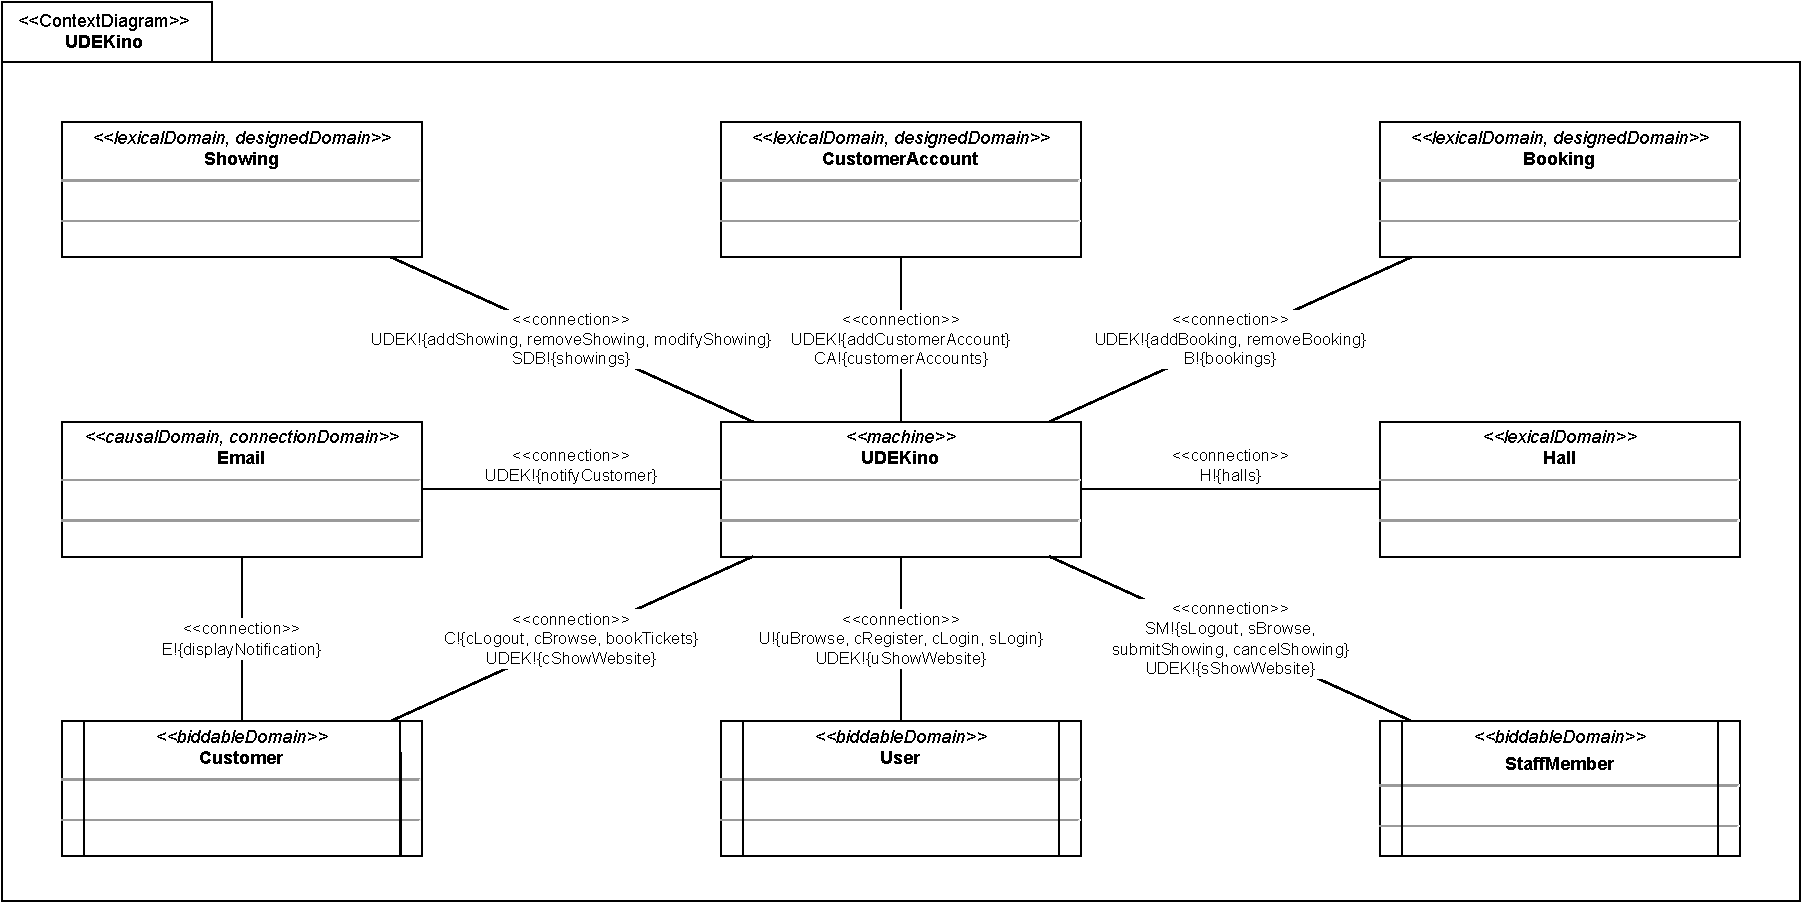
\includegraphics[width=0.9\textwidth]{figures/02/a02_context_diagram.pdf}
	\caption{Contextdiagram}
	\label{figure:contextDiagram}
\end{figure}


\newpage\section{A2}
We can derive the following problem diagrams

\begin{figure}[H]
    \centering
    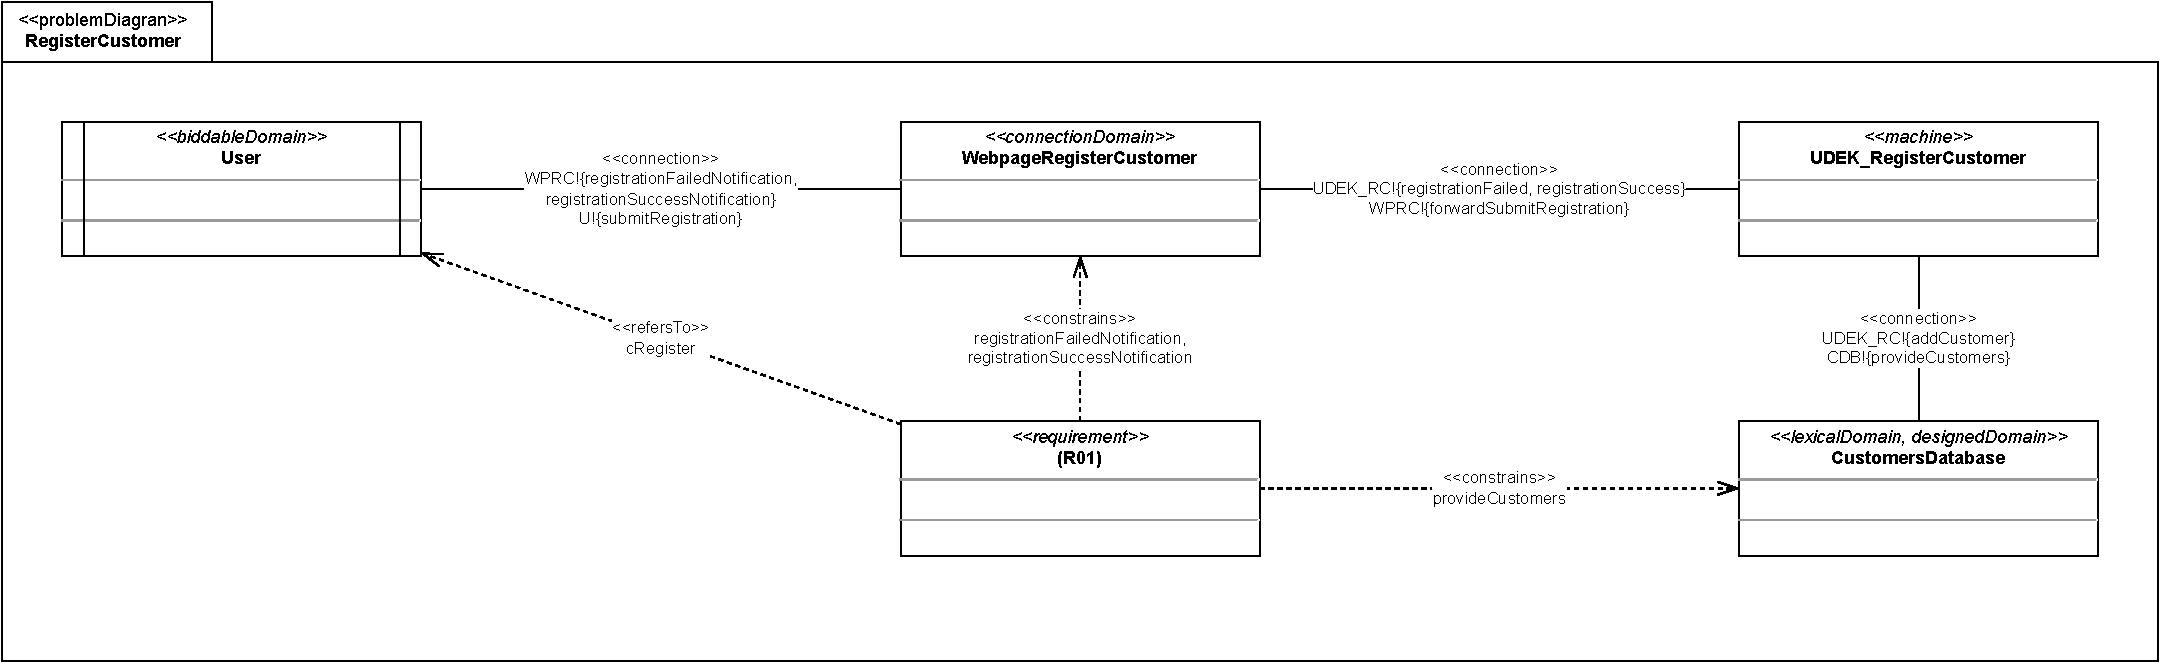
\includegraphics[width=0.9\textwidth]{figures/03/a03_problem_diagram_1-PD.pdf}
    \caption{Problem diagram for R\ref{enum:R1}}
    \label{figure:pdR1}
\end{figure}

\begin{figure}[H]
    \centering
    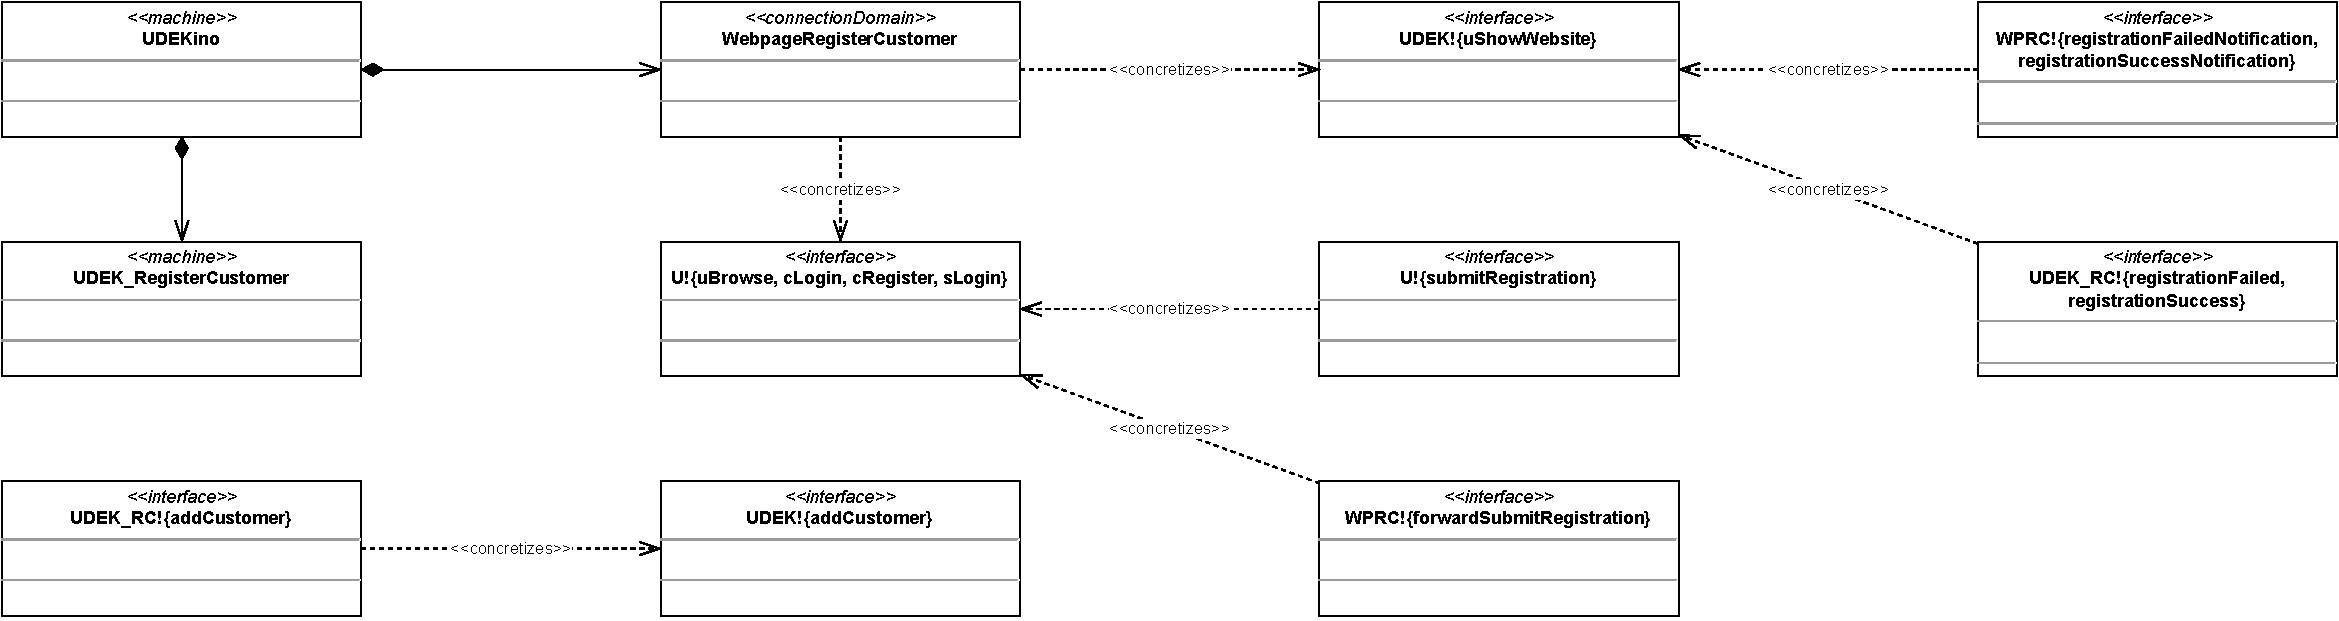
\includegraphics[width=0.9\textwidth]{figures/03/a03_problem_diagram_1-Mapping.pdf}
    \caption{Mapping diagram for R\ref{enum:R1}}
    \label{figure:mdR1}
\end{figure}

\begin{figure}[H]
    \centering
    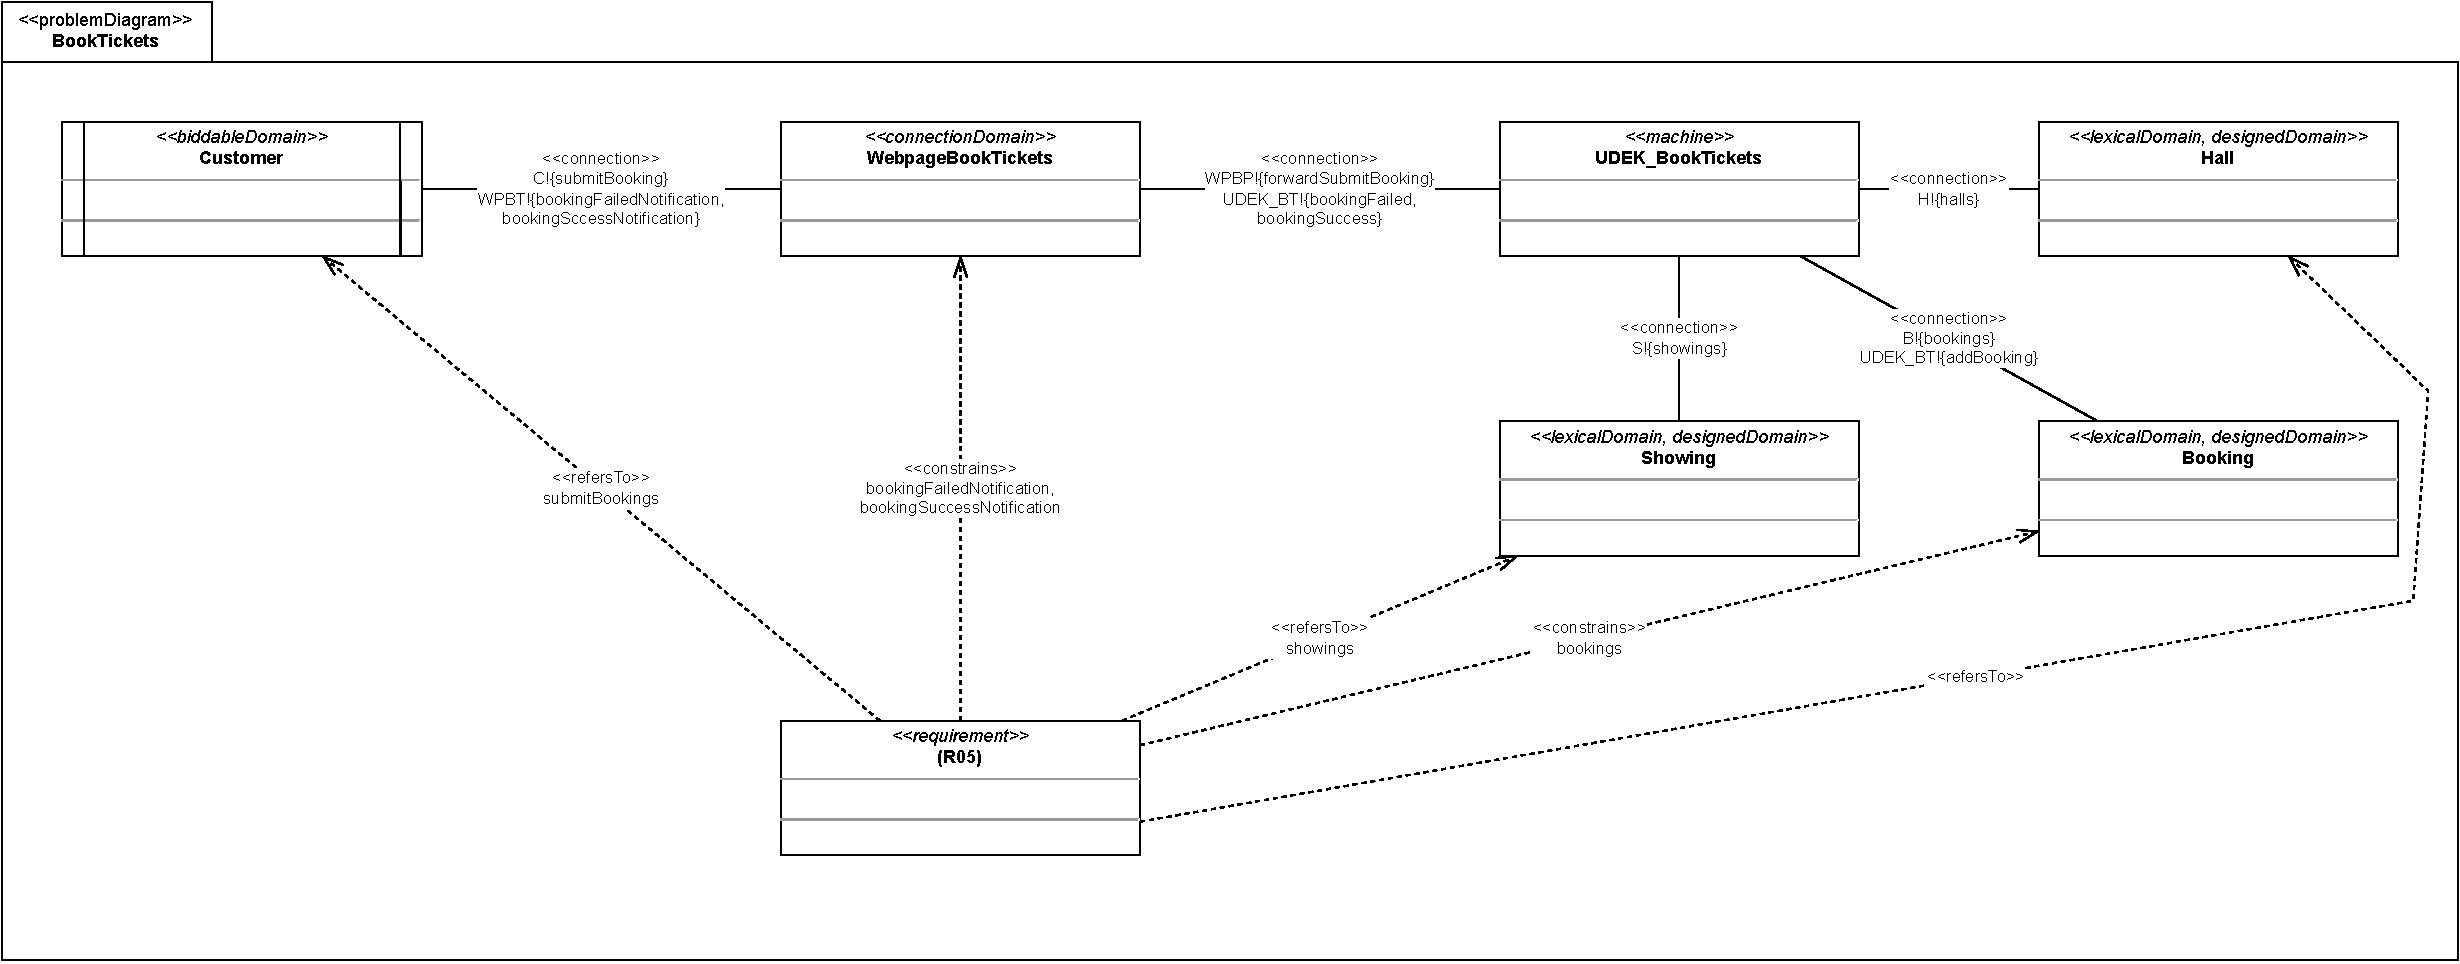
\includegraphics[width=0.9\textwidth]{figures/03/a03_problem_diagram_3-PD.pdf}
    \caption{Problem diagram for R\ref{enum:R5}}
    \label{figure:pdR5}
\end{figure}

\begin{figure}[H]
    \centering
    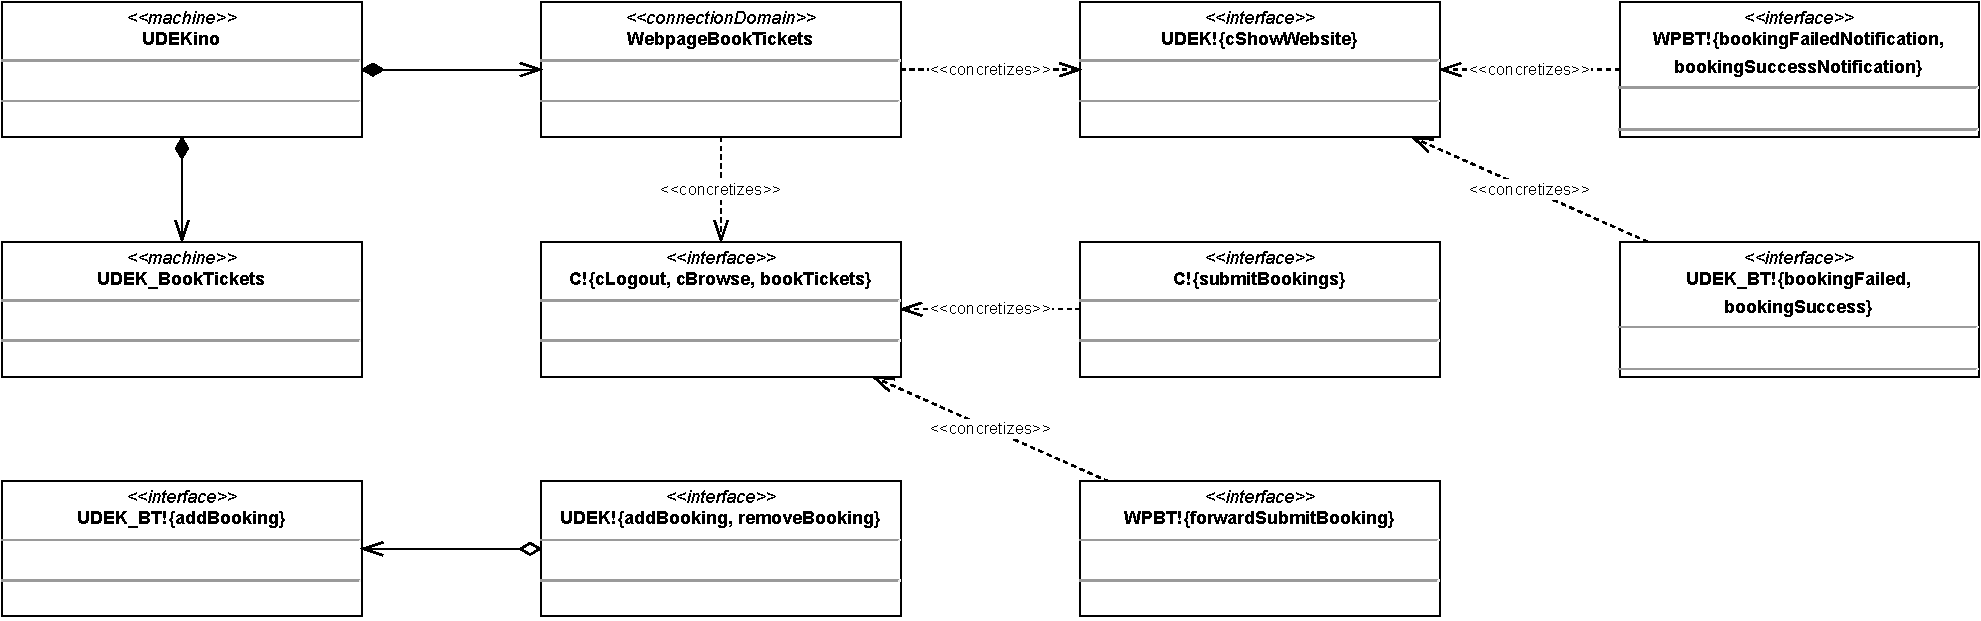
\includegraphics[width=0.9\textwidth]{figures/03/a03_problem_diagram_3-Mapping.pdf}
    \caption{Mapping diagram for R\ref{enum:R5}}
    \label{figure:mdR5}
\end{figure}

\begin{figure}[H]
\centering
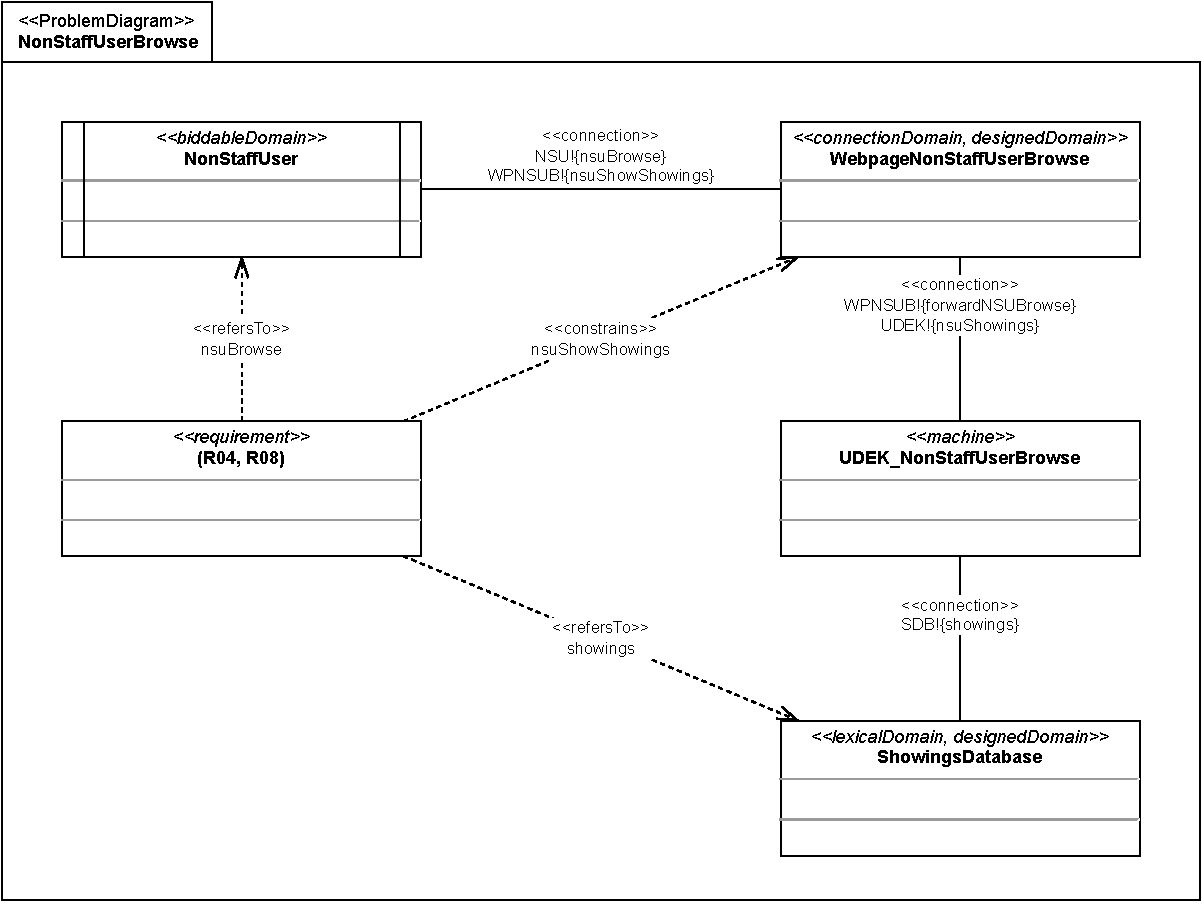
\includegraphics[width=0.9\textwidth]{figures/04/a04_problem_diagram_2-PD.pdf}
\caption{Problem diagram for R\ref{enum:R4} / R\ref{enum:R8}}
\label{figure:pdR48}
\end{figure}

\begin{figure}[H]
\centering
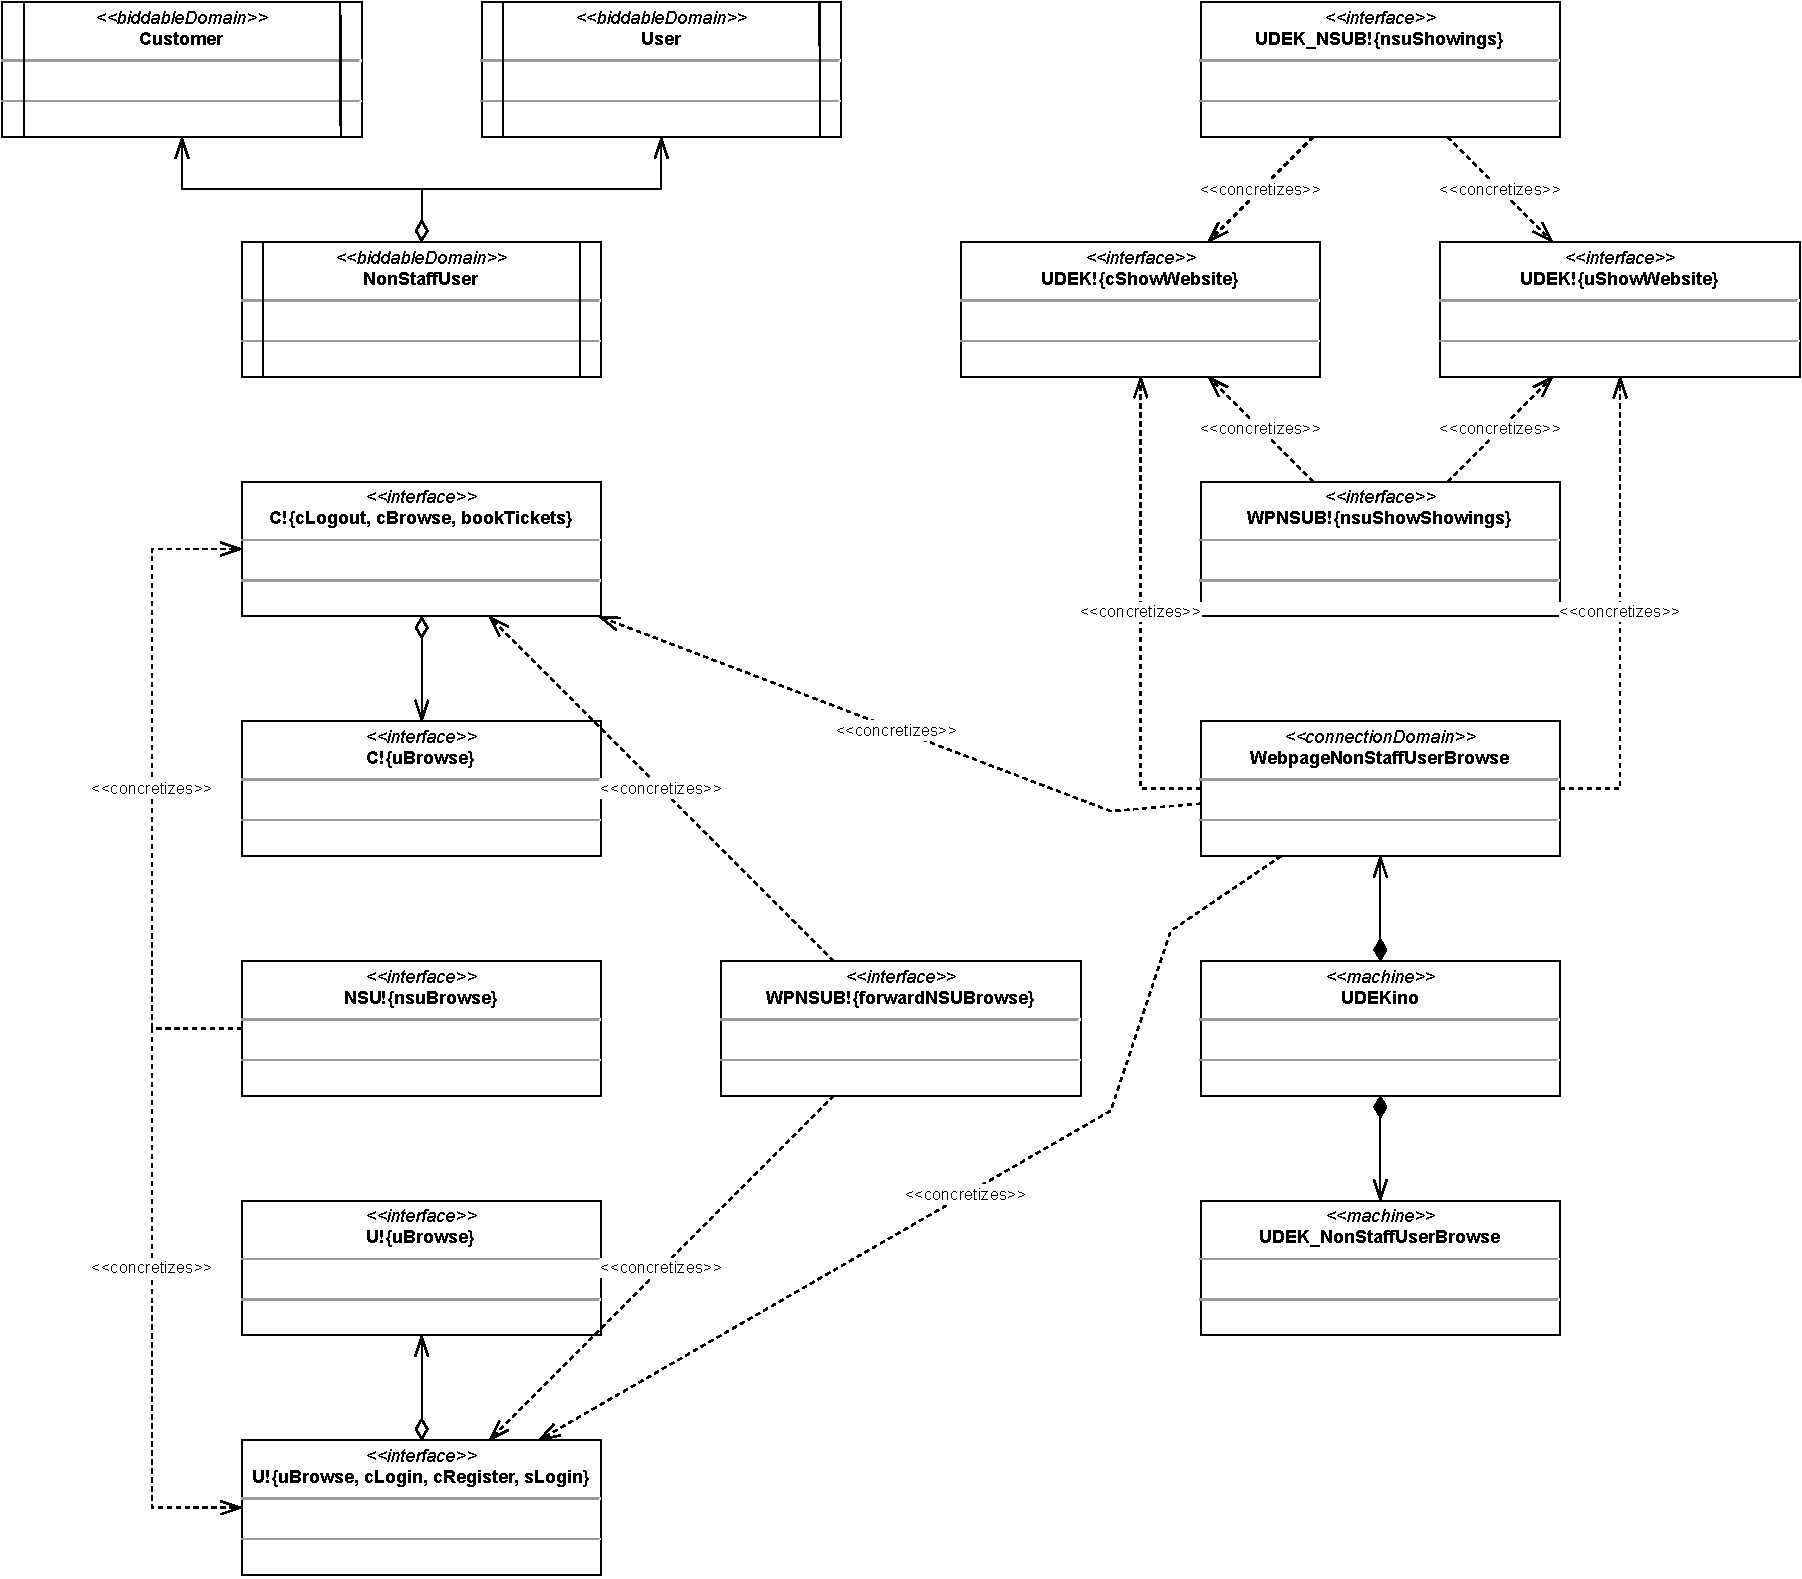
\includegraphics[width=0.9\textwidth]{figures/04/a04_problem_diagram_2-Mapping.pdf}
\caption{Mapping diagram for R\ref{enum:R4} / R\ref{enum:R8}}
\label{figure:mdR48}
\end{figure}

\begin{figure}[H]
\centering
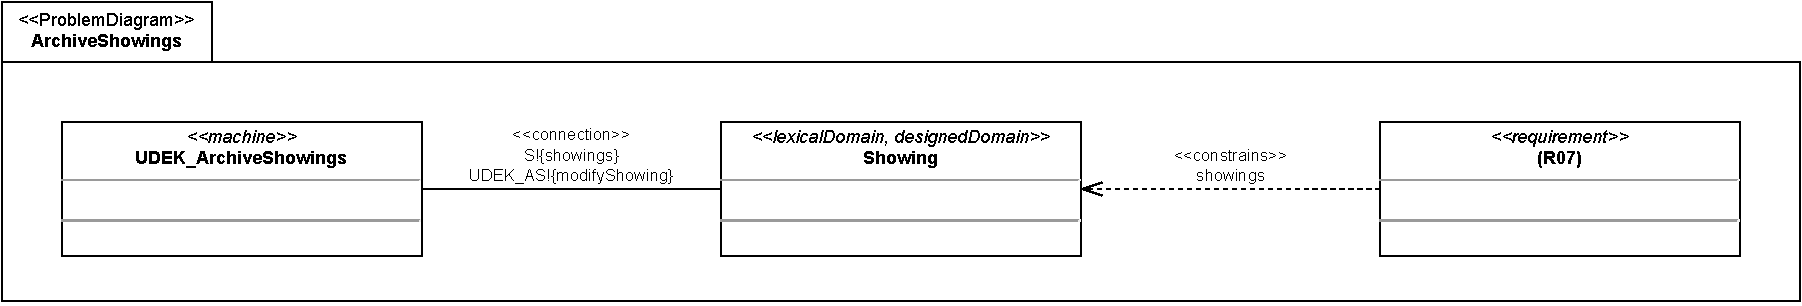
\includegraphics[width=0.9\textwidth]{figures/04/a04_problem_diagram_4-PD.pdf}
\caption{Problem diagram for R\ref{enum:R7}}
\label{figure:pdR7}
\end{figure}

\begin{figure}[H]
\centering
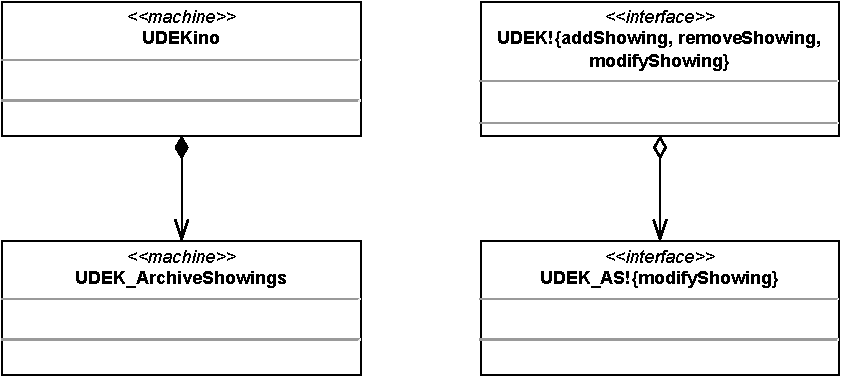
\includegraphics[width=0.9\textwidth]{figures/04/a04_problem_diagram_4-Mapping.pdf}
\caption{Mapping diagram for R\ref{enum:R7}}
\label{figure:mdR7}
\end{figure}

\subsection*{Frames}
\begin{itemize}
    \item R\ref{enum:R1} fits to update 2
    \item R\ref{enum:R5} fits to update 2
    \item R\ref{enum:R4} / R\ref{enum:R8} fits to query 2
    \item R\ref{enum:R7} fits to simple transformation
\end{itemize}

\newpage\section{A3}

\begin{figure}[H]
    \centering
    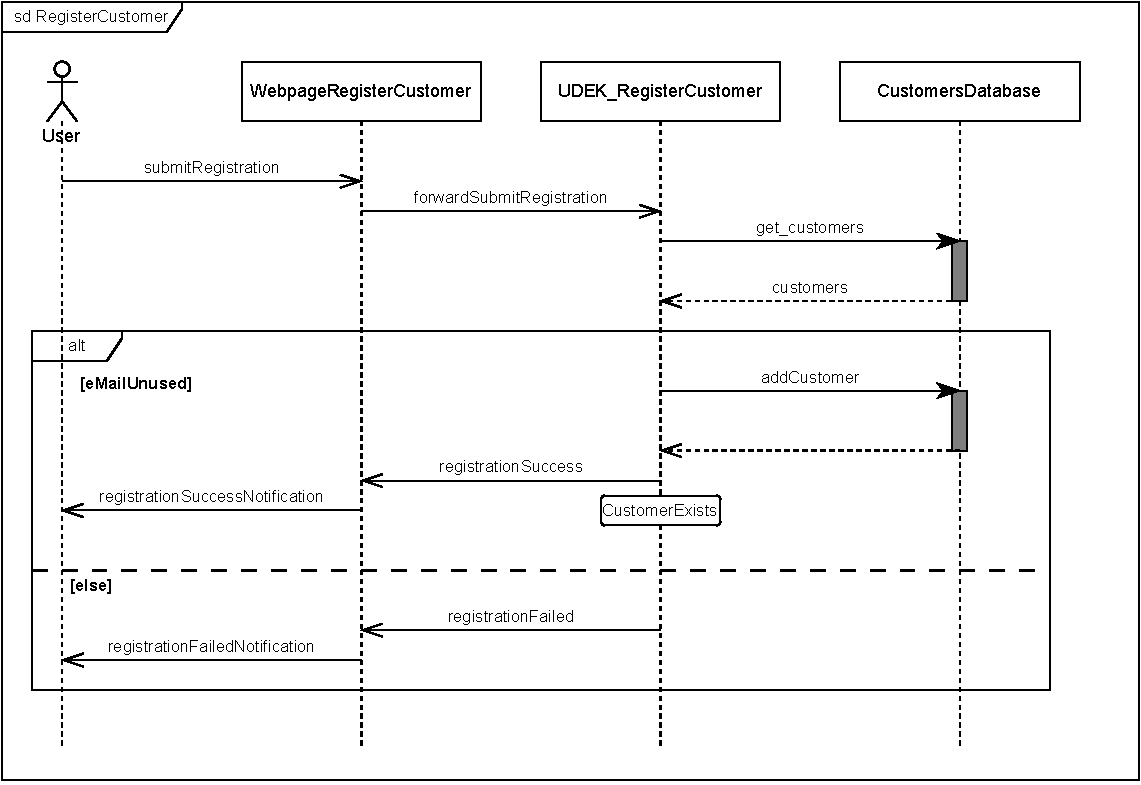
\includegraphics[width=0.9\textwidth]{figures/05/a05_sequence_diagram_r01.pdf}
    \caption{Sequence diagram for R\ref{enum:R1}}
    \label{figure:sdR1}
\end{figure}

\begin{itemize}
    \item[S1a] \textbf{WebpageRegisterCustomer}\\
    When the WebpageRegisterCustomer recieves the command "submitRegistration", the command is forwarded to machine with "forwardSubmitRegistration".
    Results are recieved via commands "registrationFailed" or "registrationSuccess" and displayed to the User via "registrationFailedNotification" / "registrationSuccessNotification".

    \item[S1b] \textbf{UDEK\_RegisterCustomer}\\
    When the machine receives the command ``fowardSubmitRegistration'' the availability of the e-mail address is checked against existing Customer accounts in the CustomerAccount database via ``get\_customerAccounts''.
    If the e-mail address is available, a new Customer account is created with the data from the forwarded request and added to the CustomerAccount database via ``addCustomerAccount'' and a confirmation is sent to the WebpageRegisterCustomer via ``registrationSuccess''.
    If the e-mail address is not available, account creation fails and a failure notification is sent to the WebpageRegisterCustomer via ``registrationFailed''.

    \item[S1c] \textbf{CustomerAccount}\\
    When the database receives the command ``get\_customerAccounts'', all Customer accounts are returned as the data ``customerAccounts''.
    When the database receives the command ``addCustomerAccount'', the Customer account is added.
\end{itemize}

$(A2) \land (S1a) \land (S1b) \land (S1c) \implies (R\ref{enum:R1})$

\begin{figure}[H]
\centering
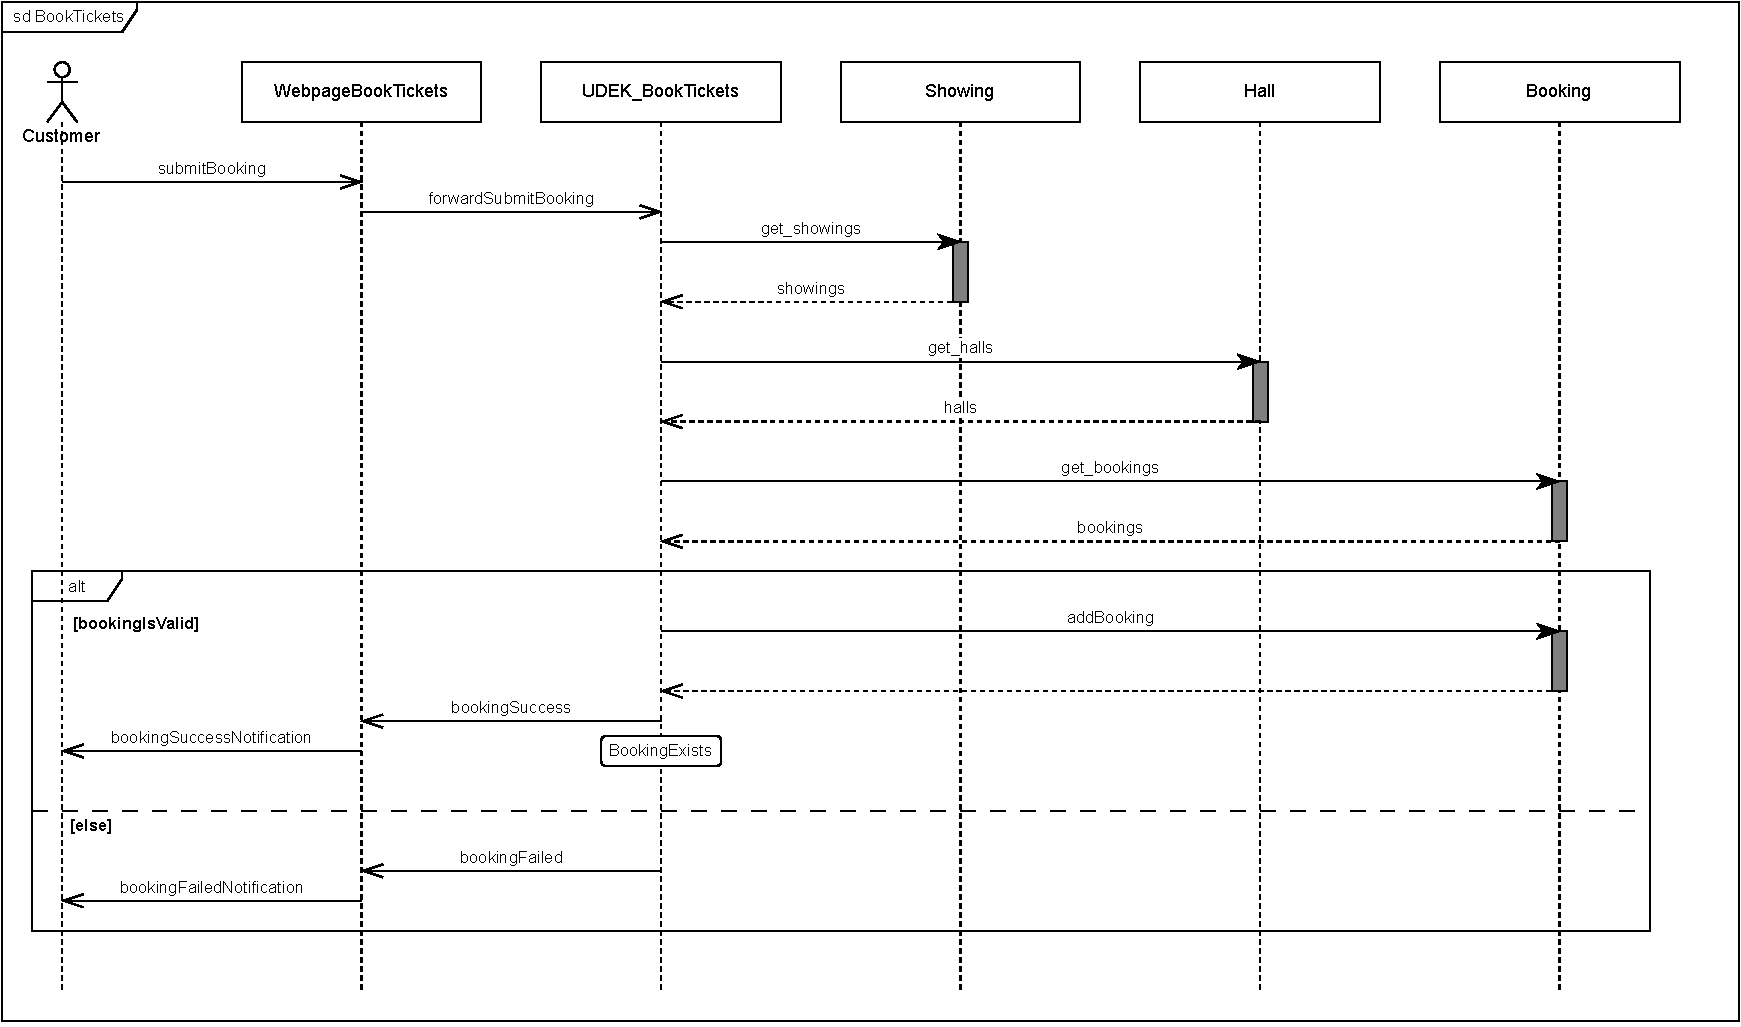
\includegraphics[width=0.9\textwidth]{figures/05/a05_sequence_diagram_r05.pdf}
\caption{Sequence diagram for R\ref{enum:R5}}
\label{figure:sdR5}
\end{figure}

\begin{itemize}
\item[S2a] \textbf{WebpageBookTickets}\\
When the Webpage receives the command ``submitBooking'', the command is forwarded to the machine with the command ``forwardSubmitBooking''.
Results are received via ``bookingFailed'' or ``bookingSuccess'' and displayed the the Customer via
``bookingFailedNotification'' / ``bookingSuccessNotification''

\item[S2b] \textbf{UDEK\_BookTickets}
When the machine receives the command ``forwardSubmitBooking'', the machine checks the availability of the desired showing and seats against the Showing database, Hall database and Booking database via ``get\_showings'', ``get\_halls'' and ``get\_bookings''.
If the desired showing and seats exist, the showing begins in more than 15 minutes and the seats are not already booked, the booking is added to the Booking database via ``addBooking'' and a success notification is sent to the WebpageBookTickets via ``bookingSuccess''.
Otherwise the booking fails and the Webpage is notified of the failure via ``bookingFailed''.

\item[S2c] \textbf{Showing}
When the database receives the command ``get\_showings'', all showings are returned as the data ``showings''.

\item[S2d] \textbf{Hall}
When the database receives the command ``get\_halls'', all halls are returned as the data ``halls''.

\item[S2c] \textbf{Booking}
When the database receives the command ``get\_bookings'', all bookings are returned as the data ``bookings''.
When the database receives the command ``addBooking'', the booking is added.

\end{itemize}

$(F3) \land (S2a) \land (S2b) \land (S2c) \land (S2d) \land (S2e) \implies (R\ref{enum:R5})$

\begin{figure}[H]
    \centering
    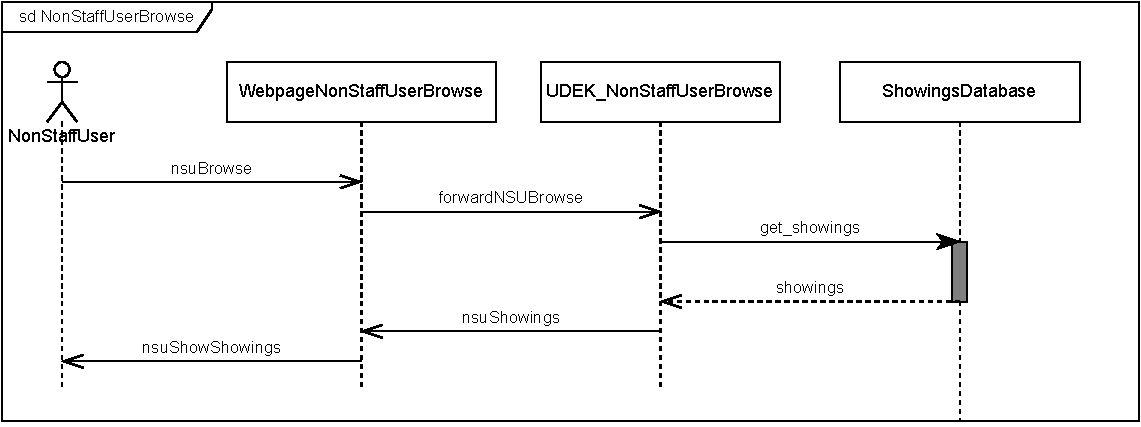
\includegraphics[width=0.9\textwidth]{figures/05/a05_sequence_diagram_r04r08.pdf}
    \caption{Sequence diagram for R\ref{enum:R4}/R\ref{enum:R8}}
    \label{figure:sdR48}
\end{figure}

\begin{itemize}
\item[S3a] \textbf{WebpageNonStaffUserBrowse}
When the Webpage receives the command ``nsuBrowse'', the command is forwarded to the machine with the command ``forwardNSUBrowse''.
Results are received via ``nsuShowings'' and displayed to NonStaffUser via ``nsuShowShowings''.

\item[S3b] \textbf{UDEK\_NonStaffUserBrowse}
When the machine receives the command "forwardNSUBrowse", the machine gets all showings from the Showing database via ``get\_showings''.
All non-archived showings are send/transfered to the Webpage via ``nsuShowings''.

\item[S3c] \textbf{Showing}
When the database receives the command ``get\_showings'', all showings are returned data as ``showings''

\end{itemize}

$(S3a) \land (S3b) \land (S3c) \implies (R\ref{enum:R4}) \land (R\ref{enum:R8})$

\begin{figure}[H]
\centering
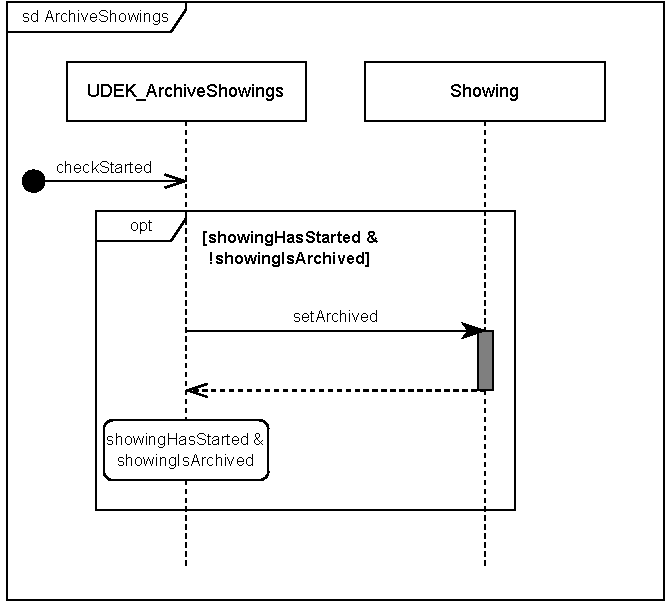
\includegraphics{figures/05/a05_sequence_diagram_r07.pdf}
\caption{Sequence diagram for R\ref{enum:R7}}
\label{figure:sdR7}
\end{figure}

\begin{itemize}
\item[S4a] \textbf{UDEK\_ArchiveShowings}
When receiving the command ``checkStarted'', all showings which have already started, and are not yet marked as archived, are marked as archived using the command ``setArchived''.

\item[S4b] \textbf{Showing}
When receiving the command ``setArchived'', all showings which have already started, and are not yet marked as archived, are marked as archived.

\end{itemize}

$(S4a) \land (S4b) \implies (R\ref{enum:R7})$

\newpage\section{A4}

\begin{figure}[H]
    \centering
    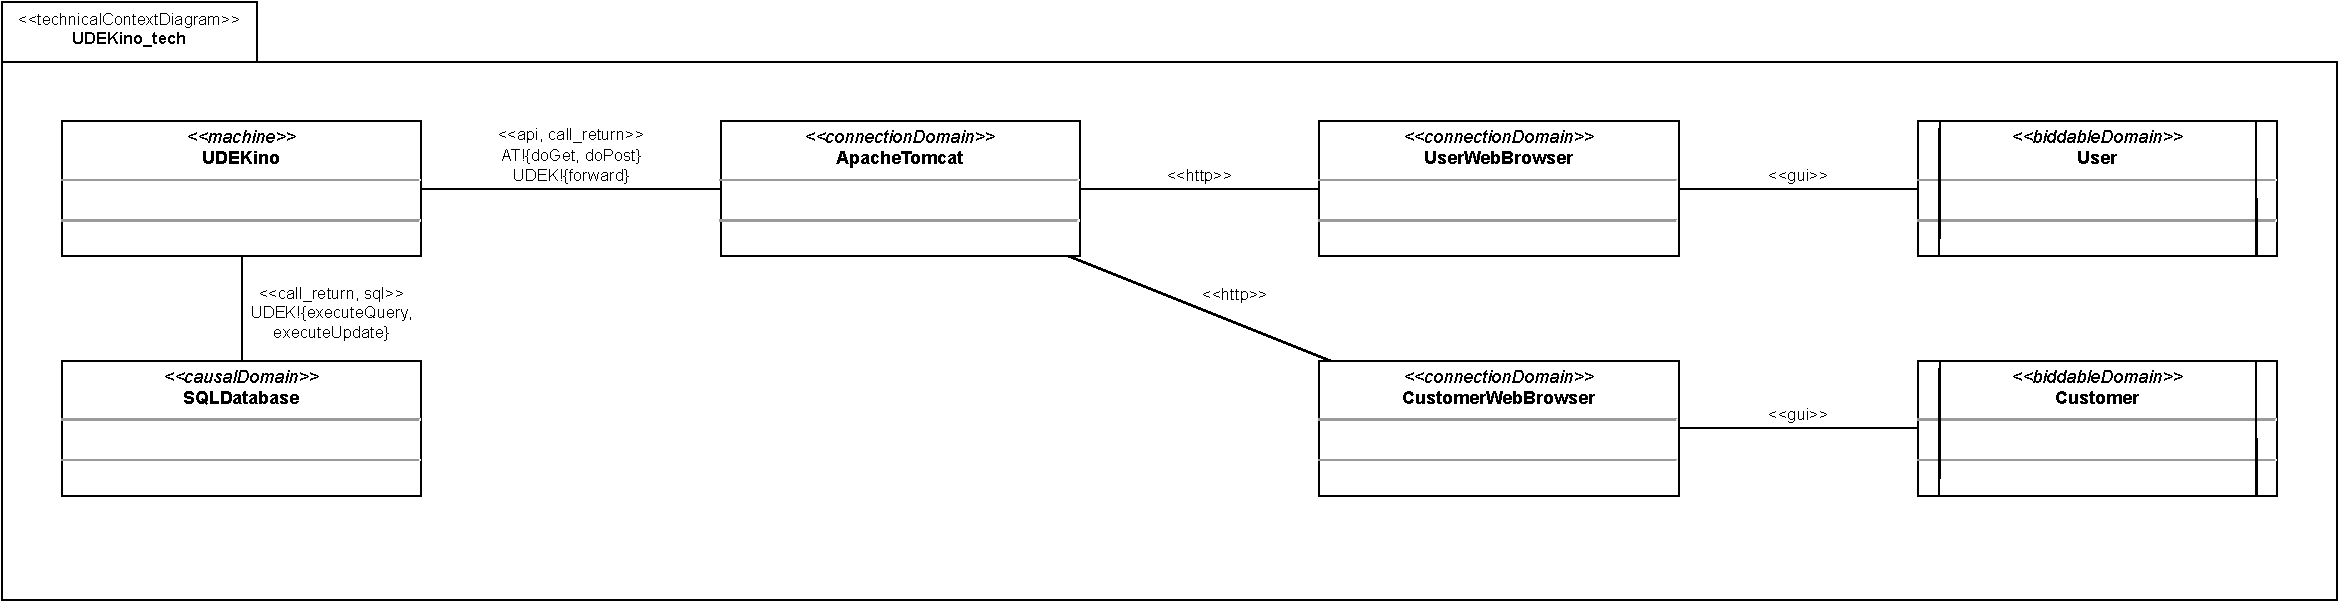
\includegraphics[width = \textwidth]{figures/06/a06_technical_context_diagram-TCD.pdf}
    \caption{Technical Context Diagram}
    \label{figure:tcd}
\end{figure}

\begin{figure}[H]
    \centering
    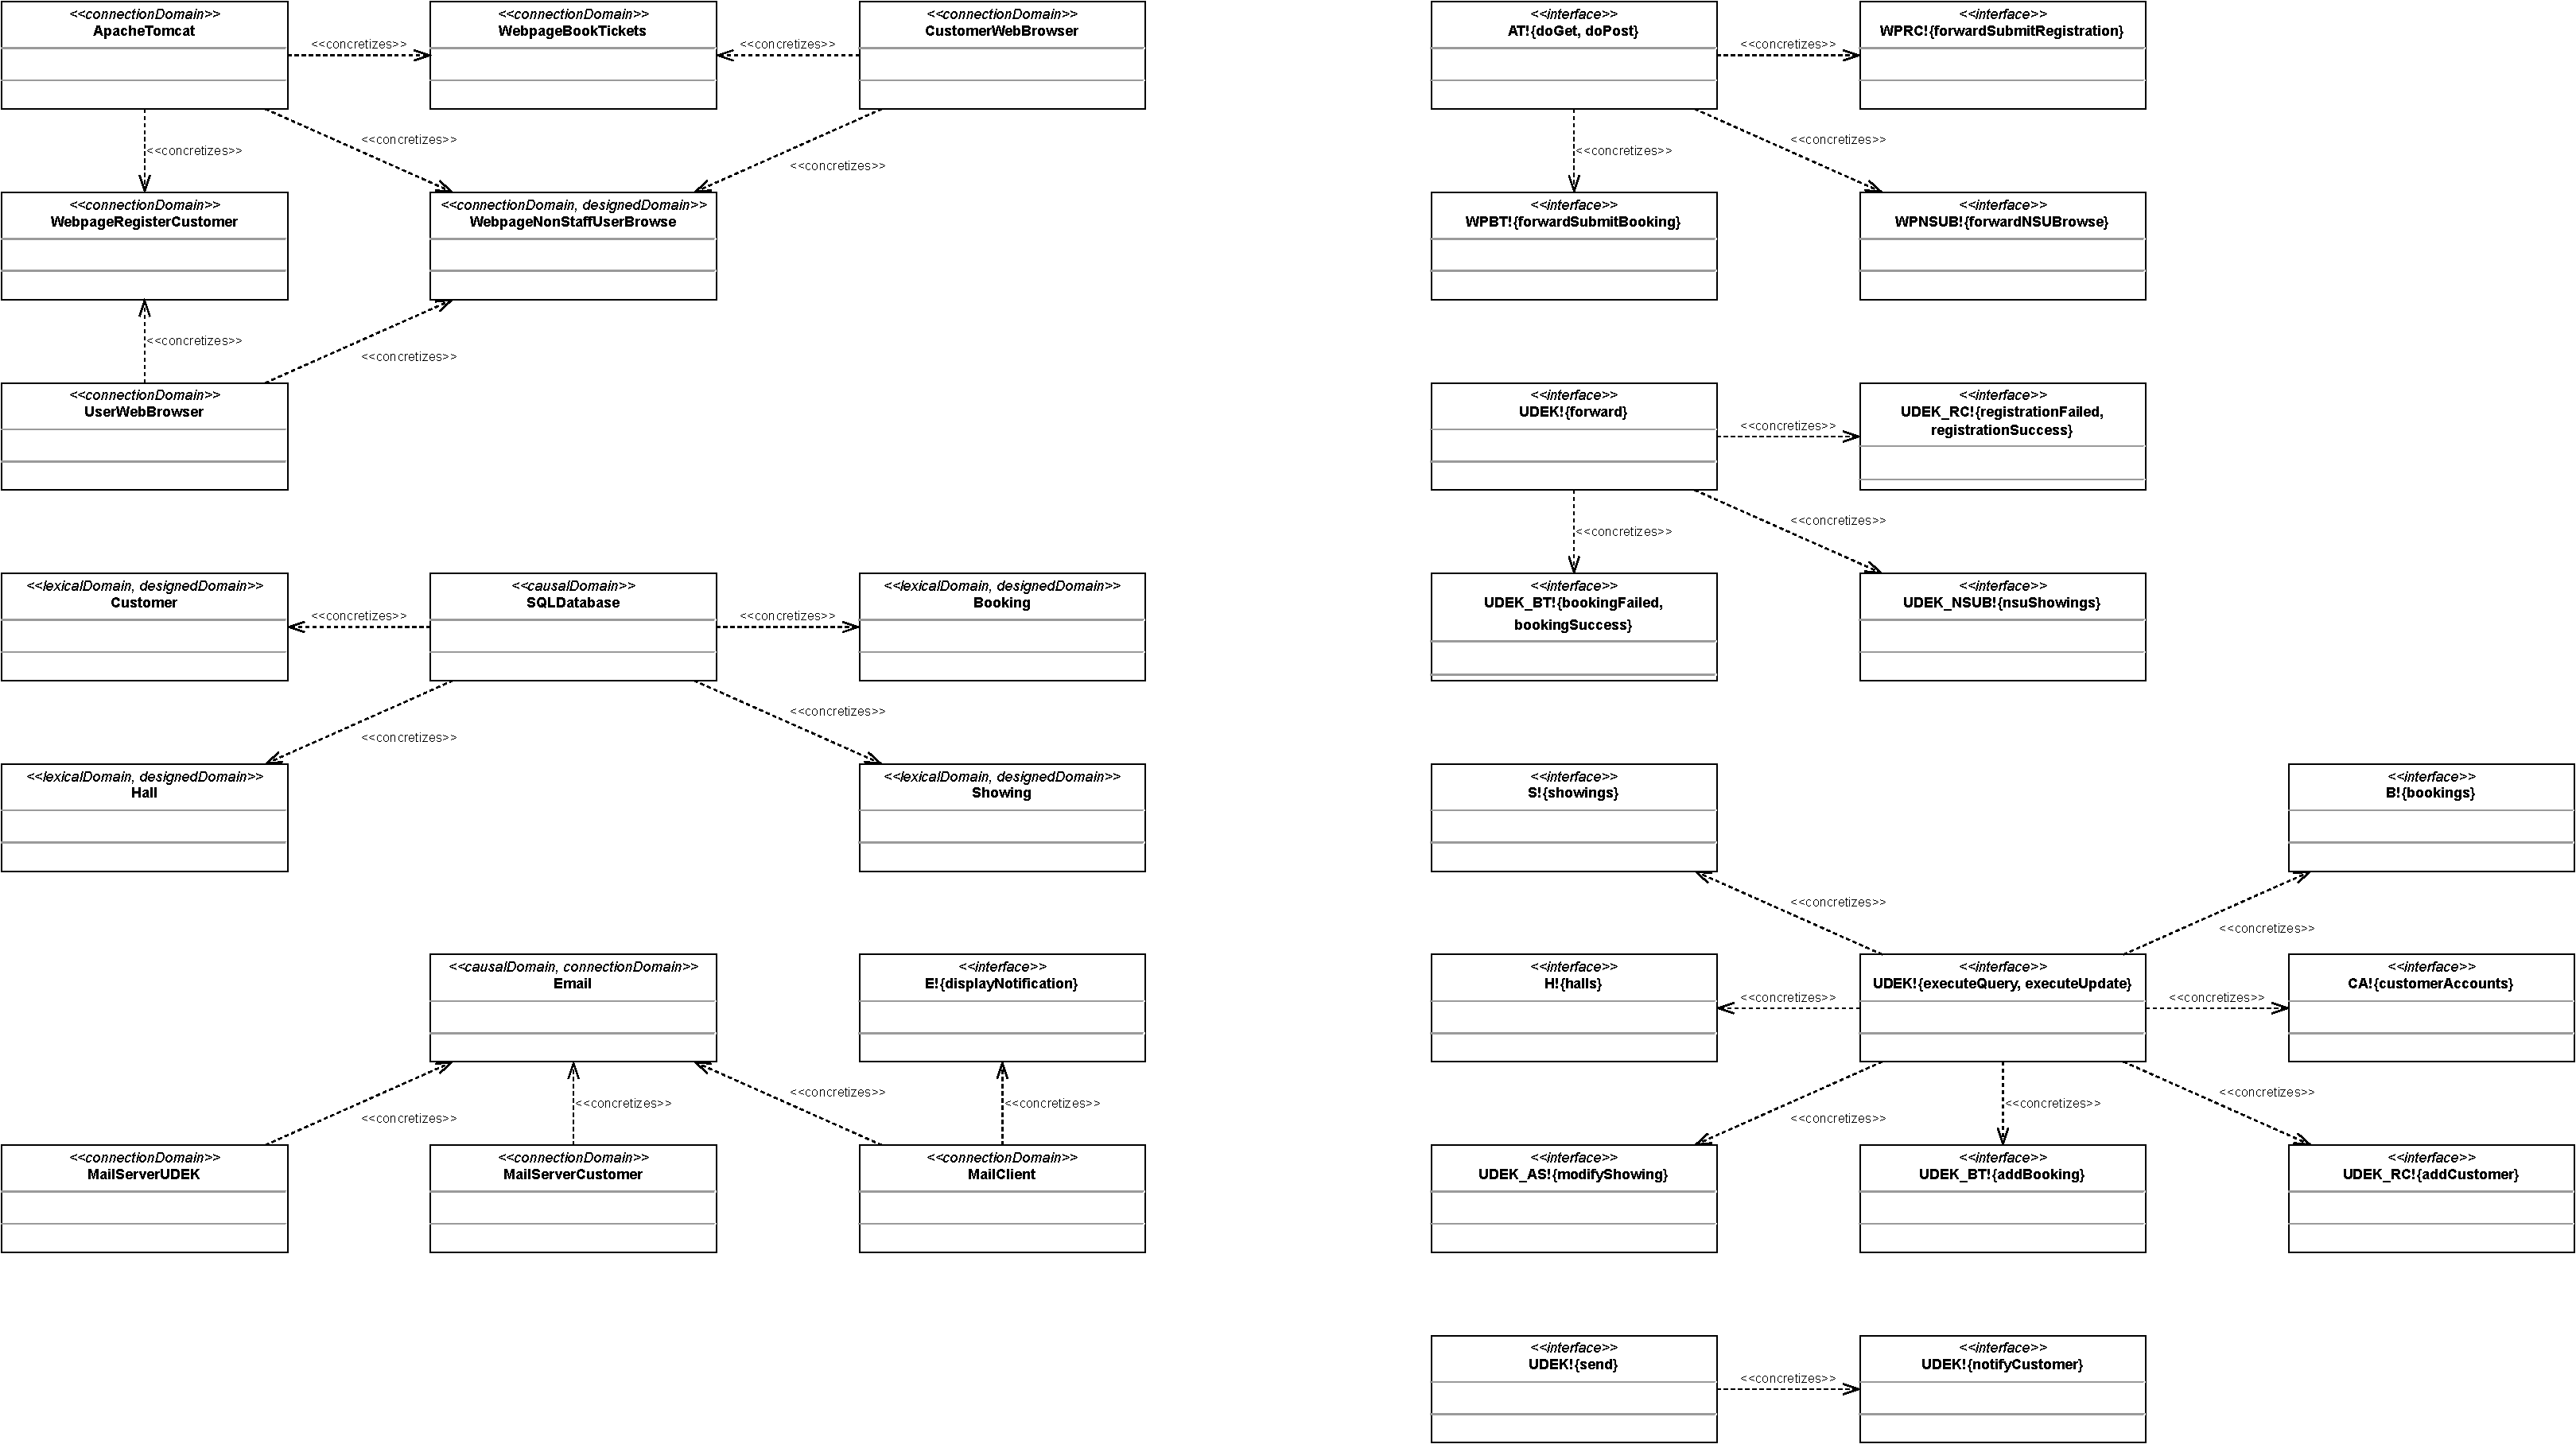
\includegraphics[width = \textwidth]{figures/06/a06_technical_context_diagram-Mapping.pdf}
    \caption{Mapping Diagram of the TCD}
    \label{figure:tcd_md}
\end{figure}

\newpage\section{A5}
%-------------------
%-------------------The following used package provides an easy OCL syntax highlighting.
%-------------------You do not have to add linebreaks. It is done automatically.
%-------------------
\lstset{language=OCL}          % Set your language (you can change the language for each code-block optionally)

\subsection{RegisterCustomer}

\begin{figure}[H]
    \centering
    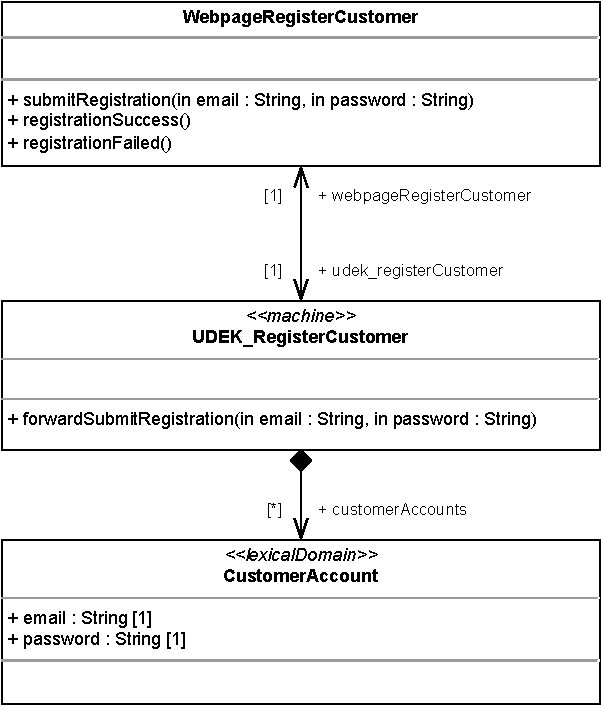
\includegraphics[]{figures/06/a06_class_diagram_RegisterCustomer.pdf}
    \caption{Class model of the operation RegisterCustomer}
    \label{figure:operation_RegisterCustomer_class_diagram}
\end{figure}

\textbf{Name:} forwardSubmitRegistration
\\
\textbf{Description:} Creates a new Customer Account with the supplied e-mail address and password and adds it to the database and then sends a success notification to the webpage, or sends a failure notification to the webpage
\\
\textbf{OCL constraint:}
\lstinputlisting[language = OCL, frame = single]{listings/a06_RegisterCustomer.ocl}

\subsection{NonStaffUserBrowse}

\begin{figure}[H]
    \centering
    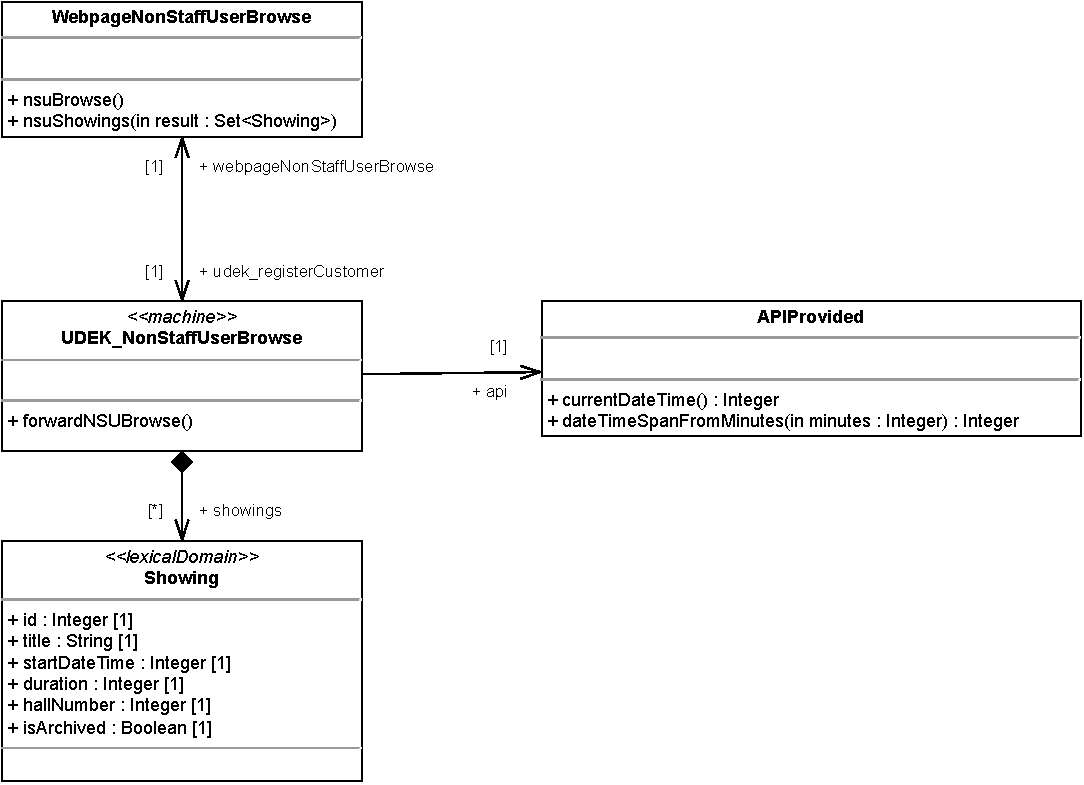
\includegraphics[width = \textwidth]{figures/06/a06_class_diagram_NonStaffUserBrowse.pdf}
    \caption{Class model of the operation NonStaffUserBrowse}
    \label{figure:operation_NonStaffUserBrowse_class_diagram}
\end{figure}

\textbf{Name:} forwardNSUBrowse
\\
\textbf{Description:} sends a set containing all showings which are not archived to the webpage
\\
\textbf{OCL constraint:}
\lstinputlisting[language = OCL, frame = single]{listings/a06_NonStaffUserBrowse.ocl}

\subsection{BookTickets}

\begin{figure}[H]
    \centering
    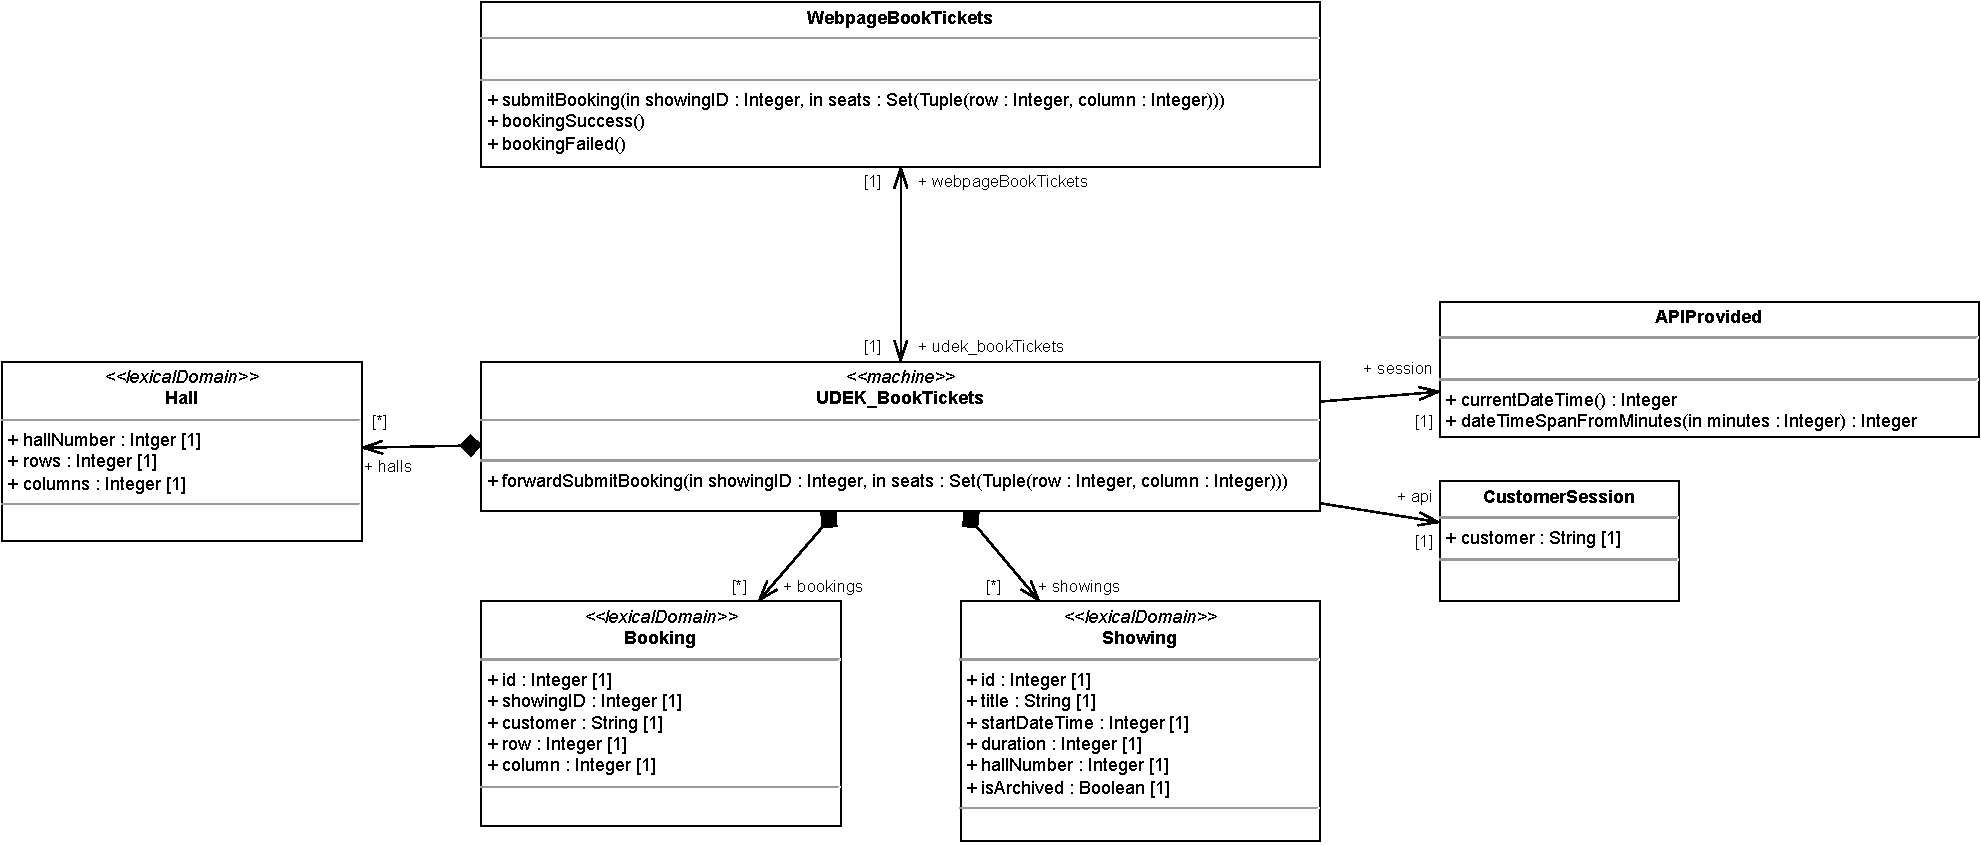
\includegraphics[width = \textwidth]{figures/07/a07_class_diagram_BookTickets.pdf}
    \caption{Class model of the operation BookTickets}
    \label{figure:operation_BookTickets_class_diagram}
\end{figure}

\textbf{Name:} forwardBookTickets
\\
\textbf{Description:} tries to book the requested seat and sends a notification whether the booking succeeded to the webpage.
\\
\textbf{OCL constraint:}
\lstinputlisting[language = OCL, frame = single]{listings/a07_BookTickets.ocl}
\textbf{Remarks}: \lstinline|CustomerSession| contains session data of the logged in customer who sent the request.

\subsection{ArchiveShowings}

\begin{figure}[H]
    \centering
    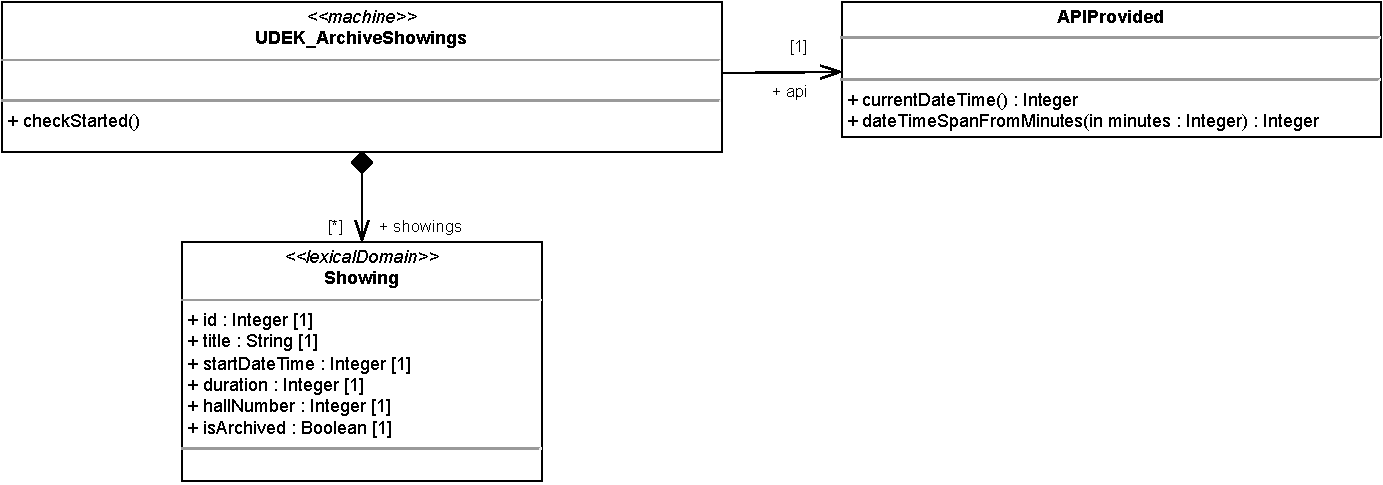
\includegraphics[width = \textwidth]{figures/07/a07_class_diagram_ArchiveShowings.pdf}
    \caption{Class model of the operation ArchiveShowings}
    \label{figure:operation_ArchiveShowings_class_diagram}
\end{figure}

\textbf{Name:} checkStarted
\\
\textbf{Description:} sets all showings which have already started as archived.
\\
\textbf{OCL constraint:}
\lstinputlisting[language = OCL, frame = single]{listings/a07_ArchiveShowings.ocl}

\newpage\section{A6}

Examples of a life-cycle using the math-environment:

$LC_{User}=(RegisterCustomer|NonStaffuserBrowse)^*$

$LC_{Customer}=(Browse^+;[Book])^*$

$LC_{NonStaffUser}=(NonStaffuserBrowse)^*$

$LC_{UDEKino}=(||_{i=1}^{n}LC_{User_i})||(||_{j=1}^{m}LC_{Customer_j})||(||_{k=1}^{l}LC_{NonStaffUser_k})||ArchiveShowings^*$



\chapter{Design}

\section{D1}

\subsection{NonStaffUserBrowse}

\begin{figure}[H]
    \centering
    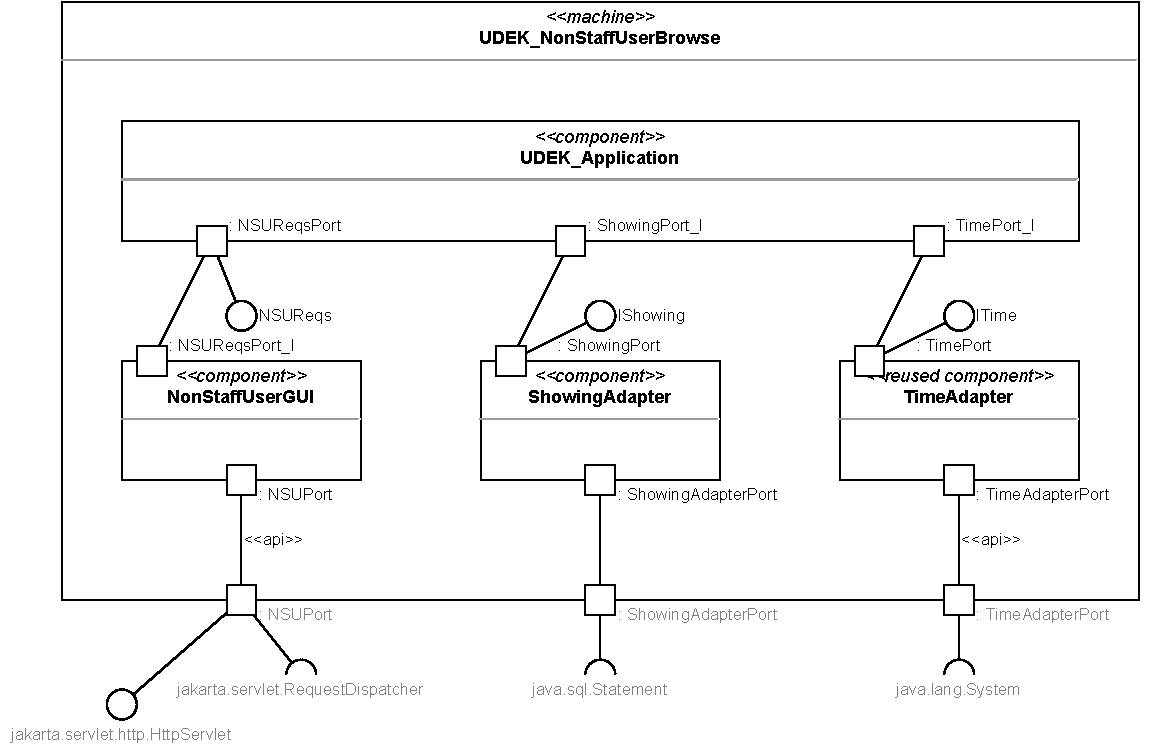
\includegraphics[width = \textwidth]{figures/08/A08_Browse-Composite Structure.drawio.pdf}
    \caption{Composite structure of NonStaffUserBrowse}
    \label{figure:NonStaffUserBrowse_composite_structure}
\end{figure}

\begin{figure}[H]
\centering
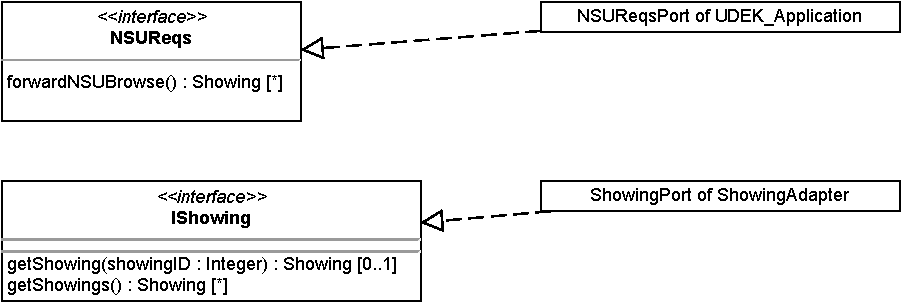
\includegraphics[width = \textwidth]{figures/08/A08_Browse-Internal Interfaces.drawio.pdf}
\caption{Internal interfaces of NonStaffUserBrowse}
\label{figure:NonStaffUserBrowse_internal_interfaces}
\end{figure}

\begin{figure}[H]
    \centering
    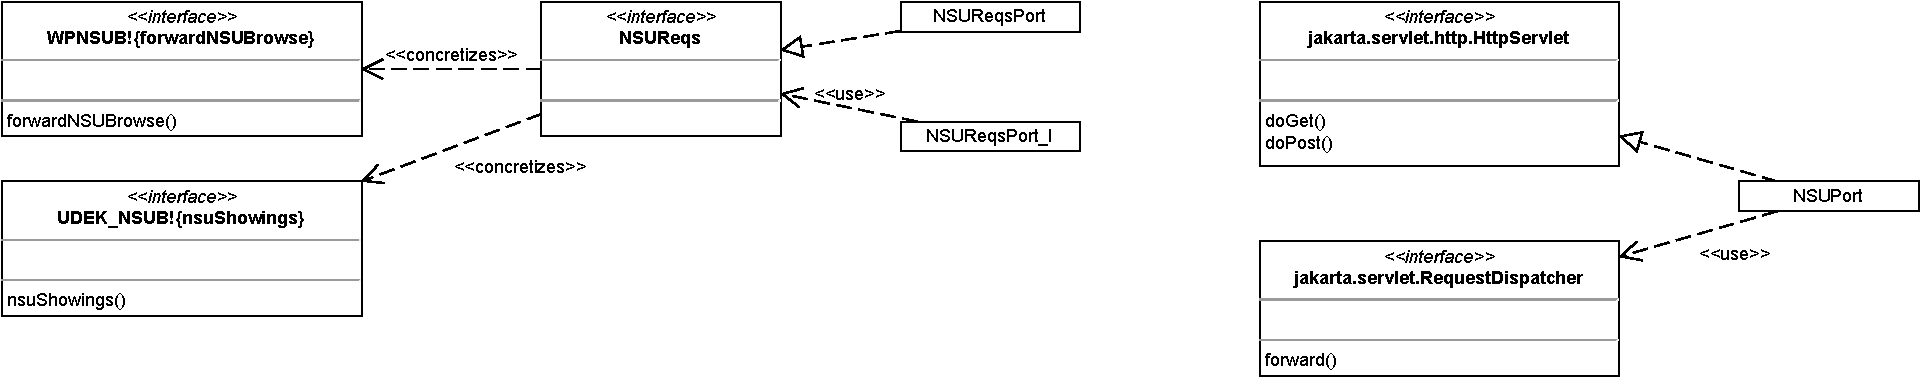
\includegraphics[width = \textwidth]{figures/08/A08_Browse-Port Types.drawio.pdf}
    \caption{Port types and interface relations of NonStaffUserBrowse}
    \label{figure:NonStaffUserBrowse_port_types}
\end{figure}

\subsection{BookTickets}

\begin{figure}[H]
\centering
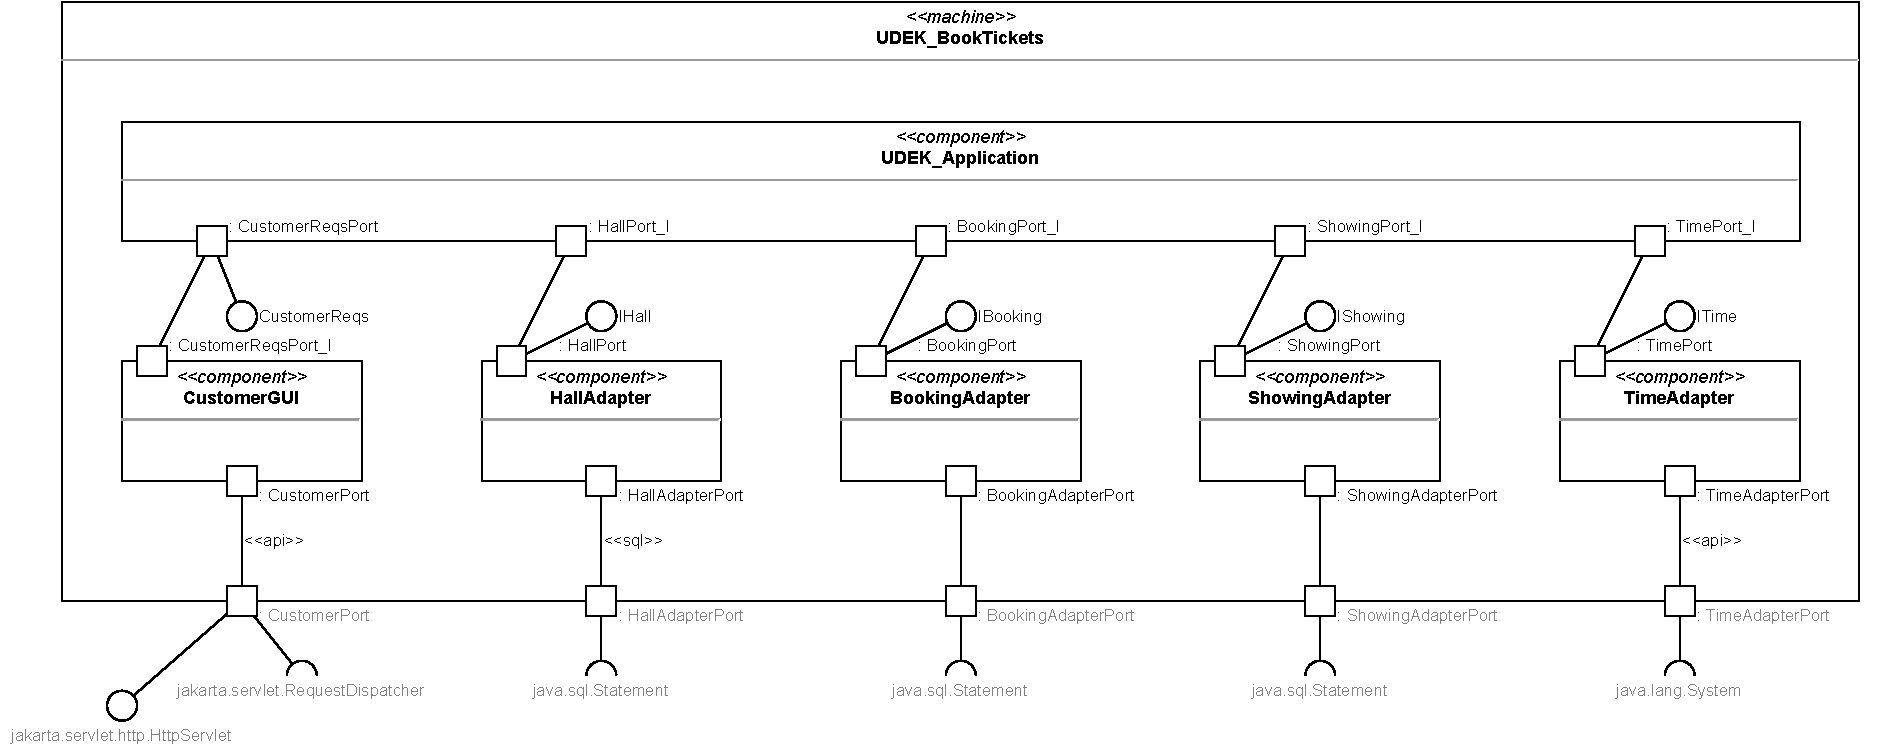
\includegraphics[width = \textwidth]{figures/08/A08_BookTickets-Composite Structure.drawio.pdf}
\caption{Composite structure of BookTickets}
\label{figure:BookTickets_composite_structure}
\end{figure}

\begin{figure}[H]
\centering
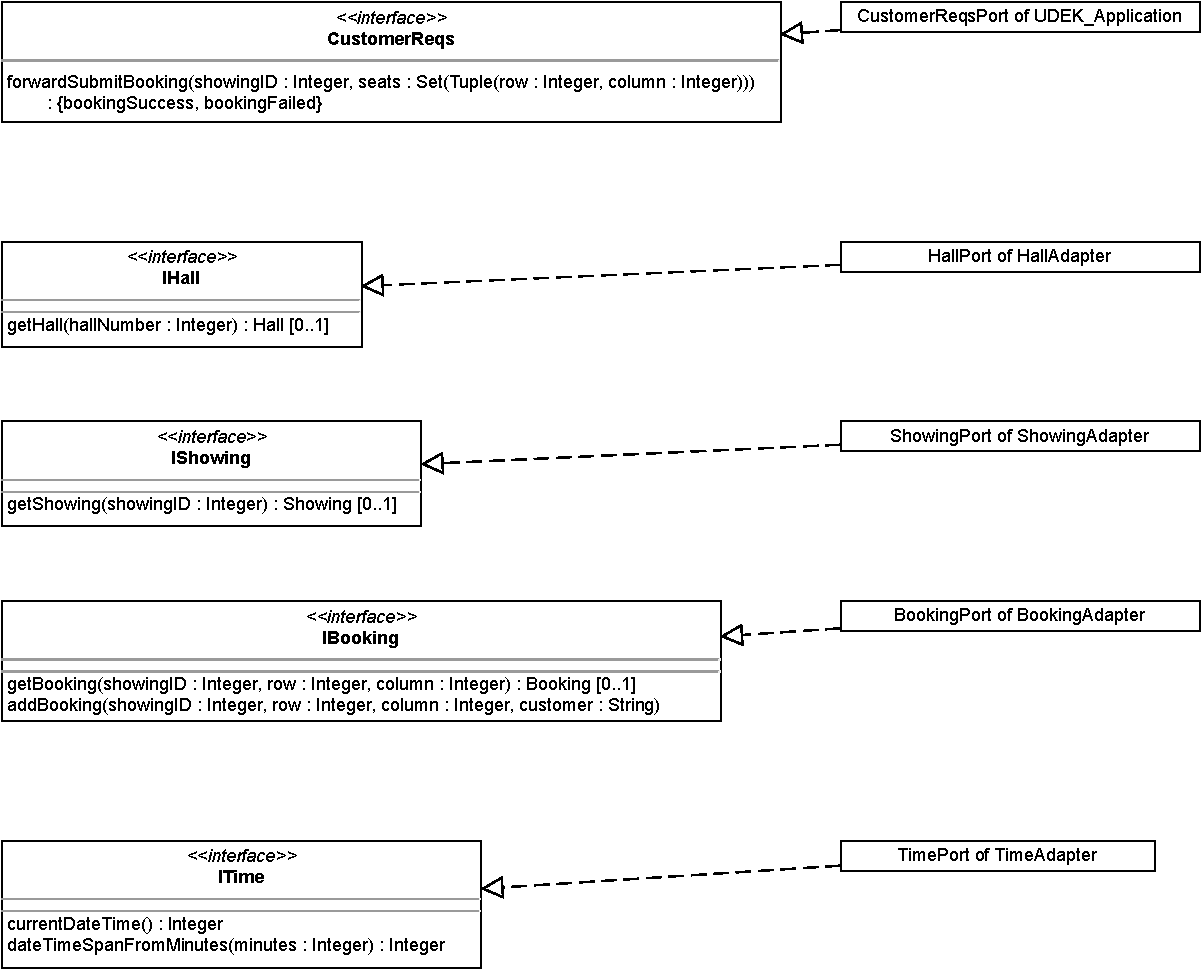
\includegraphics[width = \textwidth]{figures/08/A08_BookTickets-Internal Interfaces.drawio.pdf}
\caption{Internal interfaces of BookTickets}
\label{figure:BookTickets_internal_interfaces}
\end{figure}

\begin{figure}[H]
\centering
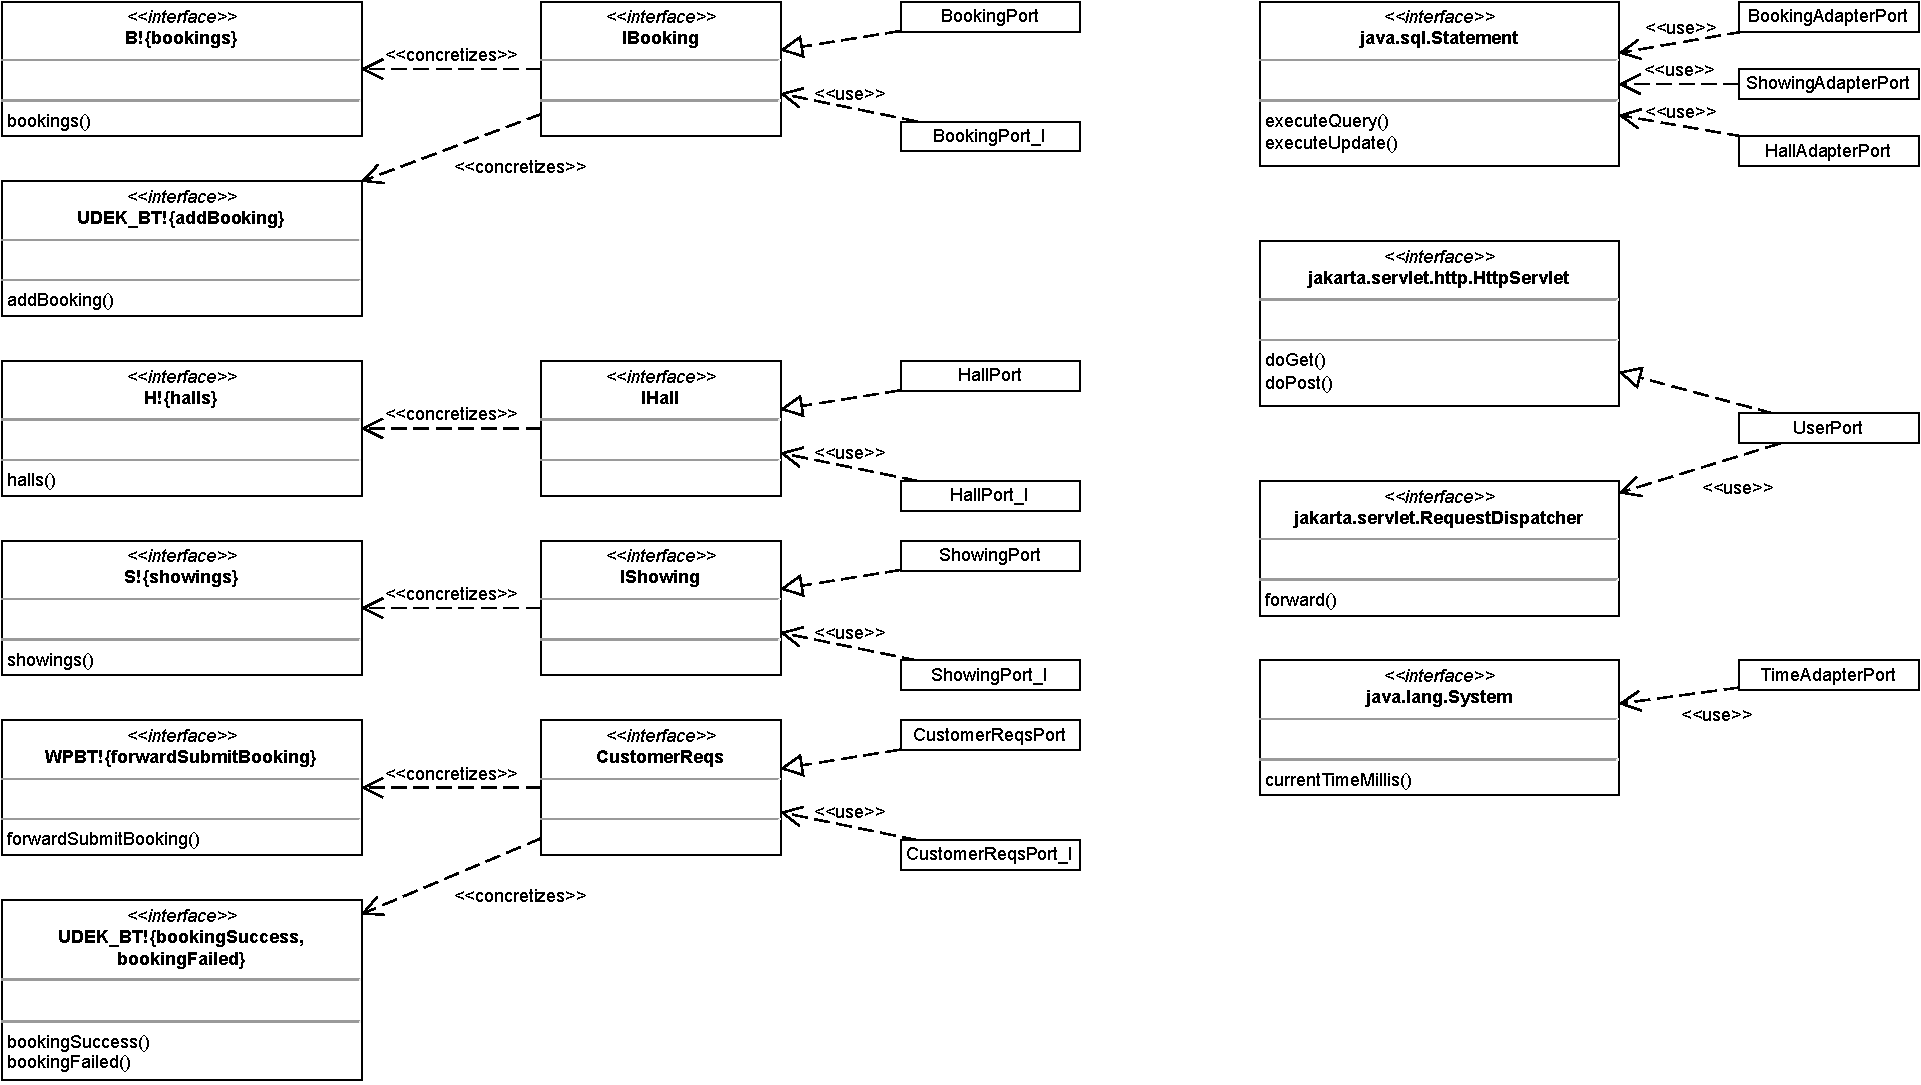
\includegraphics[width = \textwidth]{figures/08/A08_BookTickets-Port Types.drawio.pdf}
\caption{Port types and interface relations of BookTickets}
\label{figure:BookTickets_port_types}
\end{figure}

\subsection{RegisterCustomer}

\begin{figure}[H]
\centering
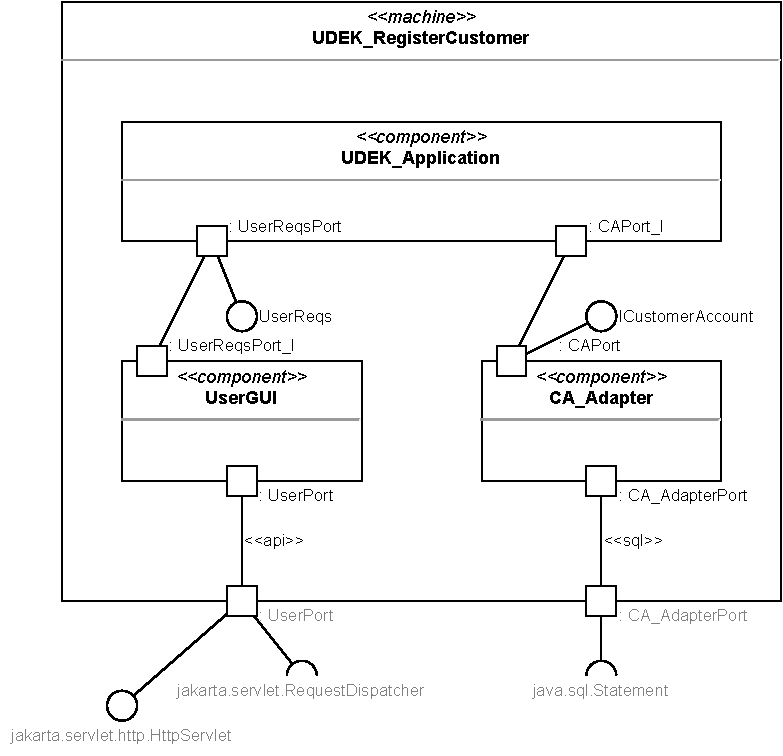
\includegraphics[width = \textwidth]{figures/08/A08_RegisterCustomer-Composite Structure.drawio.pdf}
\caption{Composite structure of RegisterCustomer}
\label{figure:RegisterCustomer_composite_structure}
\end{figure}

\begin{figure}[H]
\centering
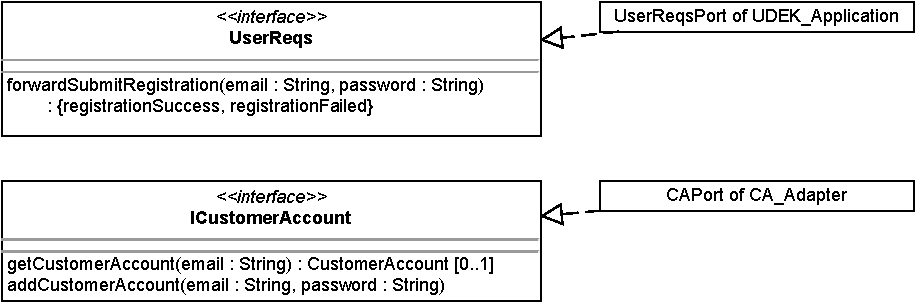
\includegraphics[width = \textwidth]{figures/08/A08_RegisterCustomer-Internal Interfaces.drawio.pdf}
\caption{Internal interfaces of RegisterCustomer}
\label{figure:RegisterCustomer_internal_interfaces}
\end{figure}

\begin{figure}[H]
\centering
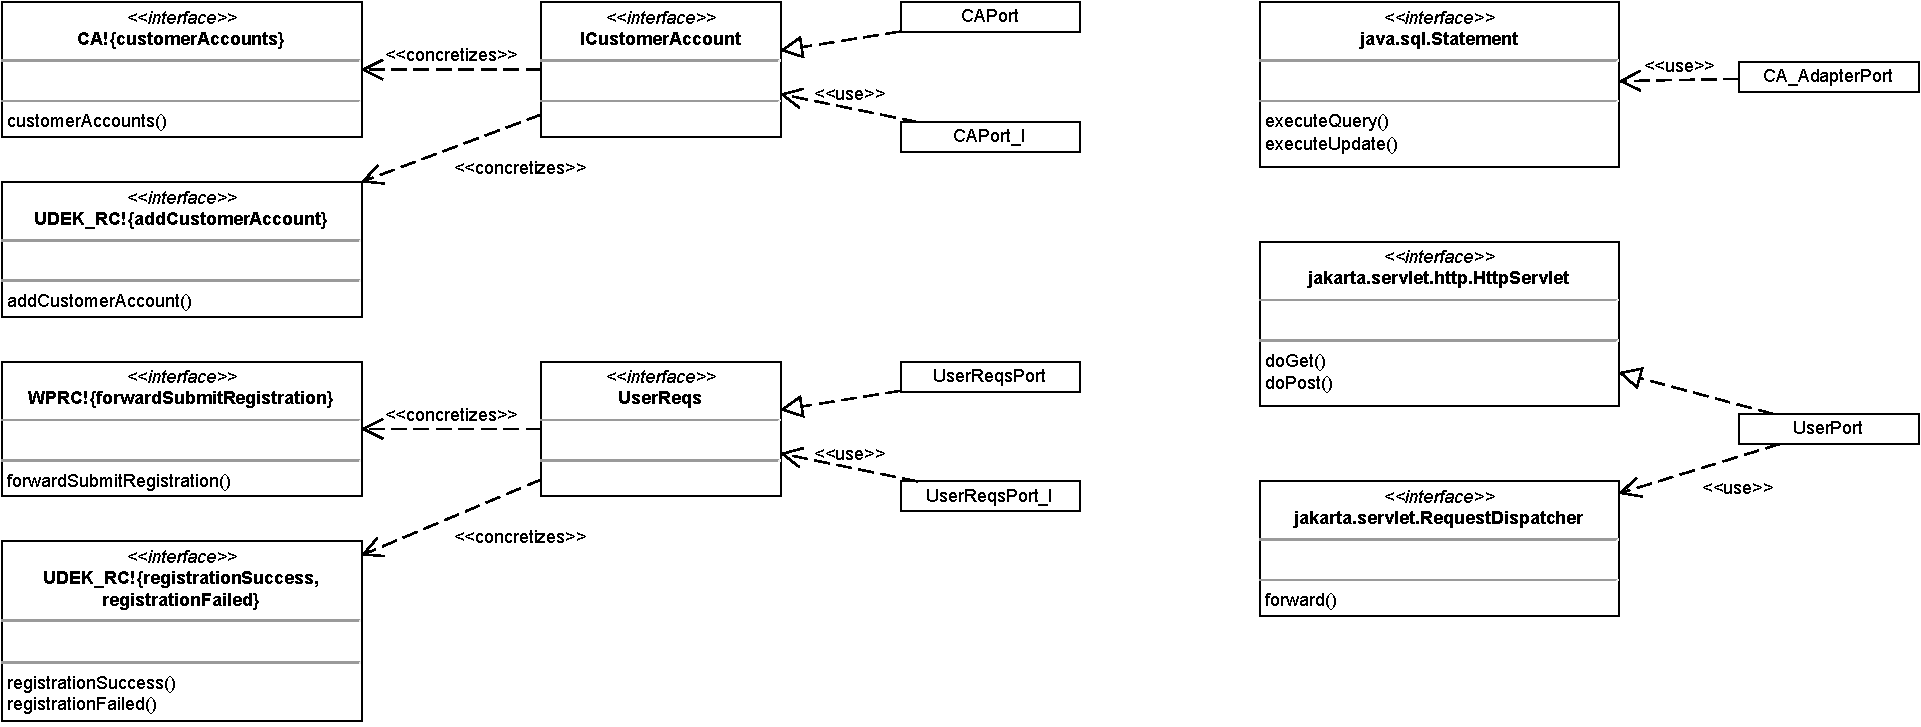
\includegraphics[width = \textwidth]{figures/08/A08_RegisterCustomer-Port Types.drawio.pdf}
\caption{Port types and interface relations of RegisterCustomer}
\label{figure:RegisterCustomer_port_types}
\end{figure}

\subsection{ArchiveShowings}

\begin{figure}[H]
\centering
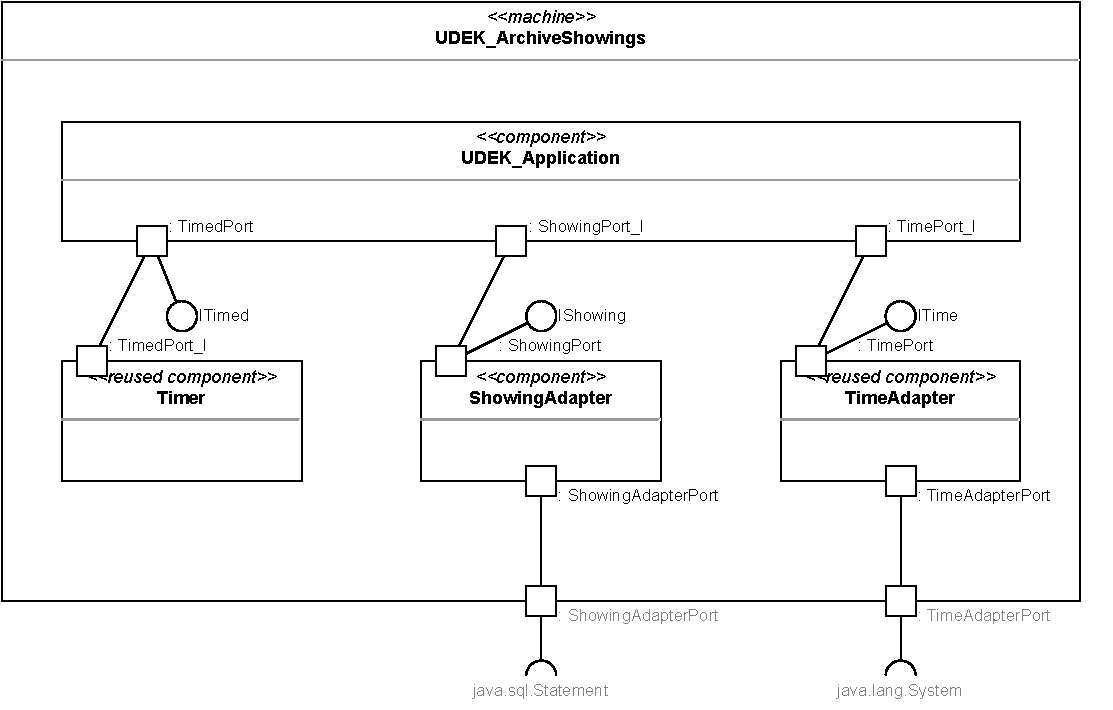
\includegraphics[width = \textwidth]{figures/08/A08_Archive-Composite Structure.drawio.pdf}
\caption{Composite structure of ArchiveShowings}
\label{figure:ArchiveShowings_composite_structure}
\end{figure}

\begin{figure}[H]
\centering
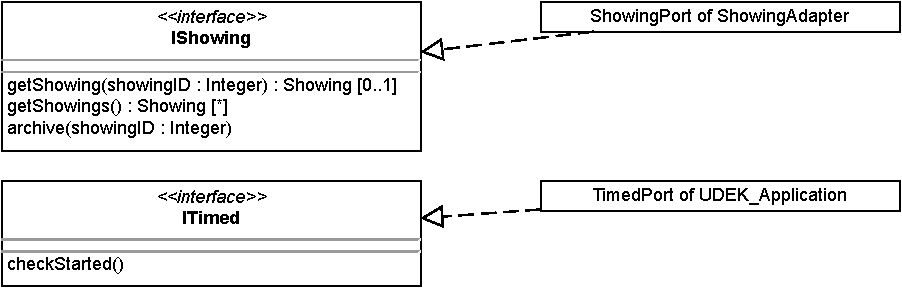
\includegraphics[width = \textwidth]{figures/08/A08_Archive-Internal Interfaces.drawio.pdf}
\caption{Internal interfaces of ArchiveShowings}
\label{figure:ArchiveShowings_internal_interfaces}
\end{figure}

\begin{figure}[H]
\centering
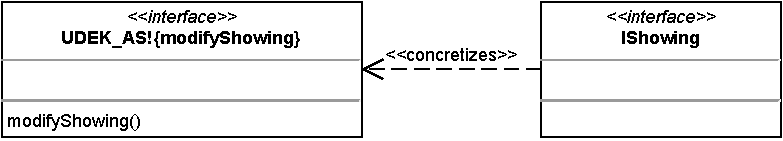
\includegraphics[width = \textwidth]{figures/08/A08_Archive-Port Types.drawio.pdf}
\caption{Port types and interface relations of ArchiveShowings}
\label{figure:ArchiveShowings_port_types}
\end{figure}

\subsection*{app\_if}
\begin{figure}[H]
    \centering
    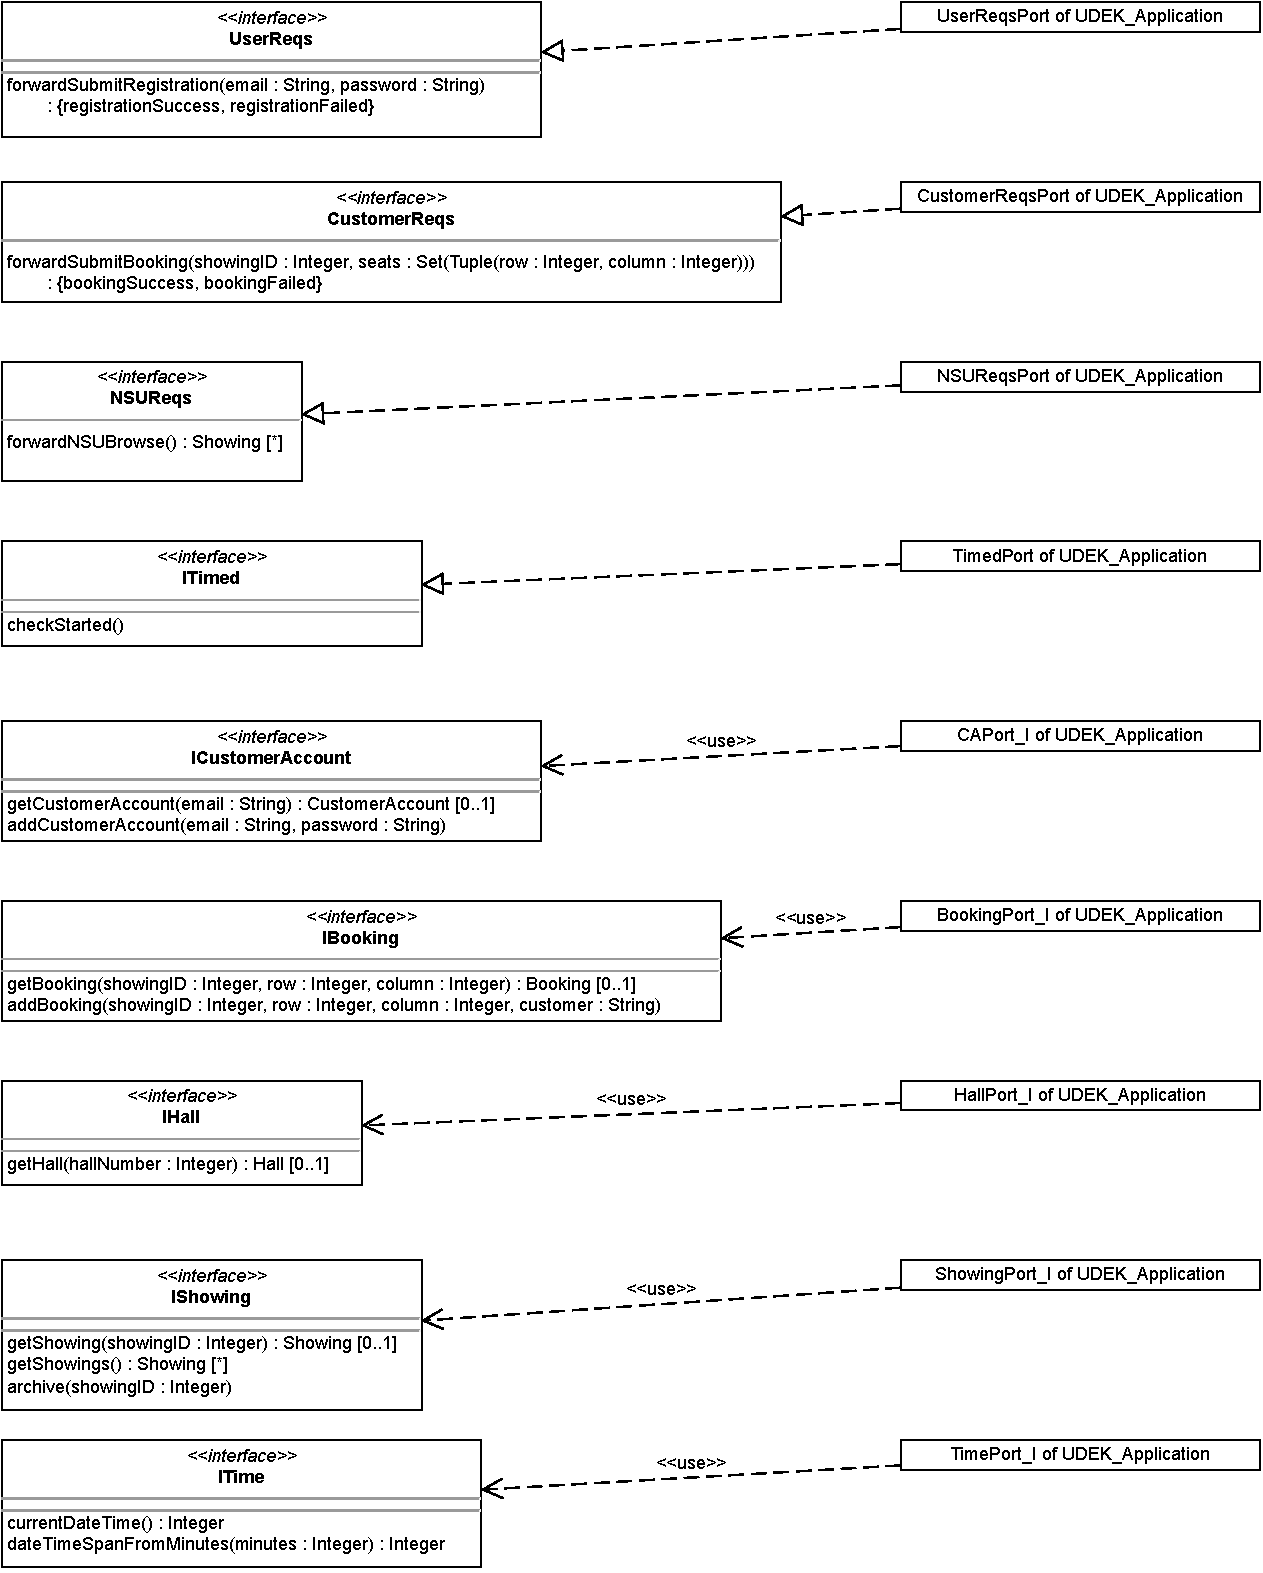
\includegraphics[width = \textwidth]{figures/08/A08_app_if.pdf}
    \caption{Port types and interface relations of ArchiveShowings}
    \label{figure:app_if}
\end{figure}

\subsection*{adapter\_if'}

There are no HAL components in the subproblem architectures. Hence, there are no \textbf{adapter\_if'} interface classes that need to be refined.

\subsection*{tech\_if''}

\begin{table}[H]
    \centering
    \begin{tabular}{|p{0.5\linewidth}|p{0.5\linewidth}|}
        \hline
        \textbf{Considered interface in subproblem architecture} & \textbf{technical interface} \\\hline\hline
        \textless\textless api\textgreater\textgreater\ jakarta.servlet.http.HttpServlet in UDEK\_NonStaffUserBrowse, UDEK\_BookTickets, UDEK\_RegisterCustomer
        & \textless\textless api, call\_return\textgreater\textgreater\ AT!\{doGet, doPost\}
        \\\hline
        \textless\textless api\textgreater\textgreater\ jakarta.servlet.RequestDispatcher in UDEK\_NonStaffUserBrowse, UDEK\_BookTickets, UDEK\_RegisterCustomer
        & \textless\textless api, call\_return\textgreater\textgreater\ UDEK!\{forward\}
        \\\hline
        \textless\textless api\textgreater\textgreater\ java.sql.Statement in UDEK\_NonStaffUserBrowse, UDEK\_BookTickets, UDEK\_RegisterCustomer, UDEK\_ArchiveShowings
        & \textless\textless api, call\_return\textgreater\textgreater\ AT!\{executeQuery, executeUpdate\}
        \\\hline
        \textless\textless api\textgreater\textgreater\ java.lang.System in UDEK\_NonStaffUserBrowse, UDEK\_BookTickets, UDEK\_ArchiveShowings
        & omitted in the technical context diagram
        \\\hline
    \end{tabular}
    \caption{tech\_if'' by TCD}
    \label{tab:tech_if}
\end{table}

\subsection{Global Architecture}
\begin{figure}[H]
    \centering
    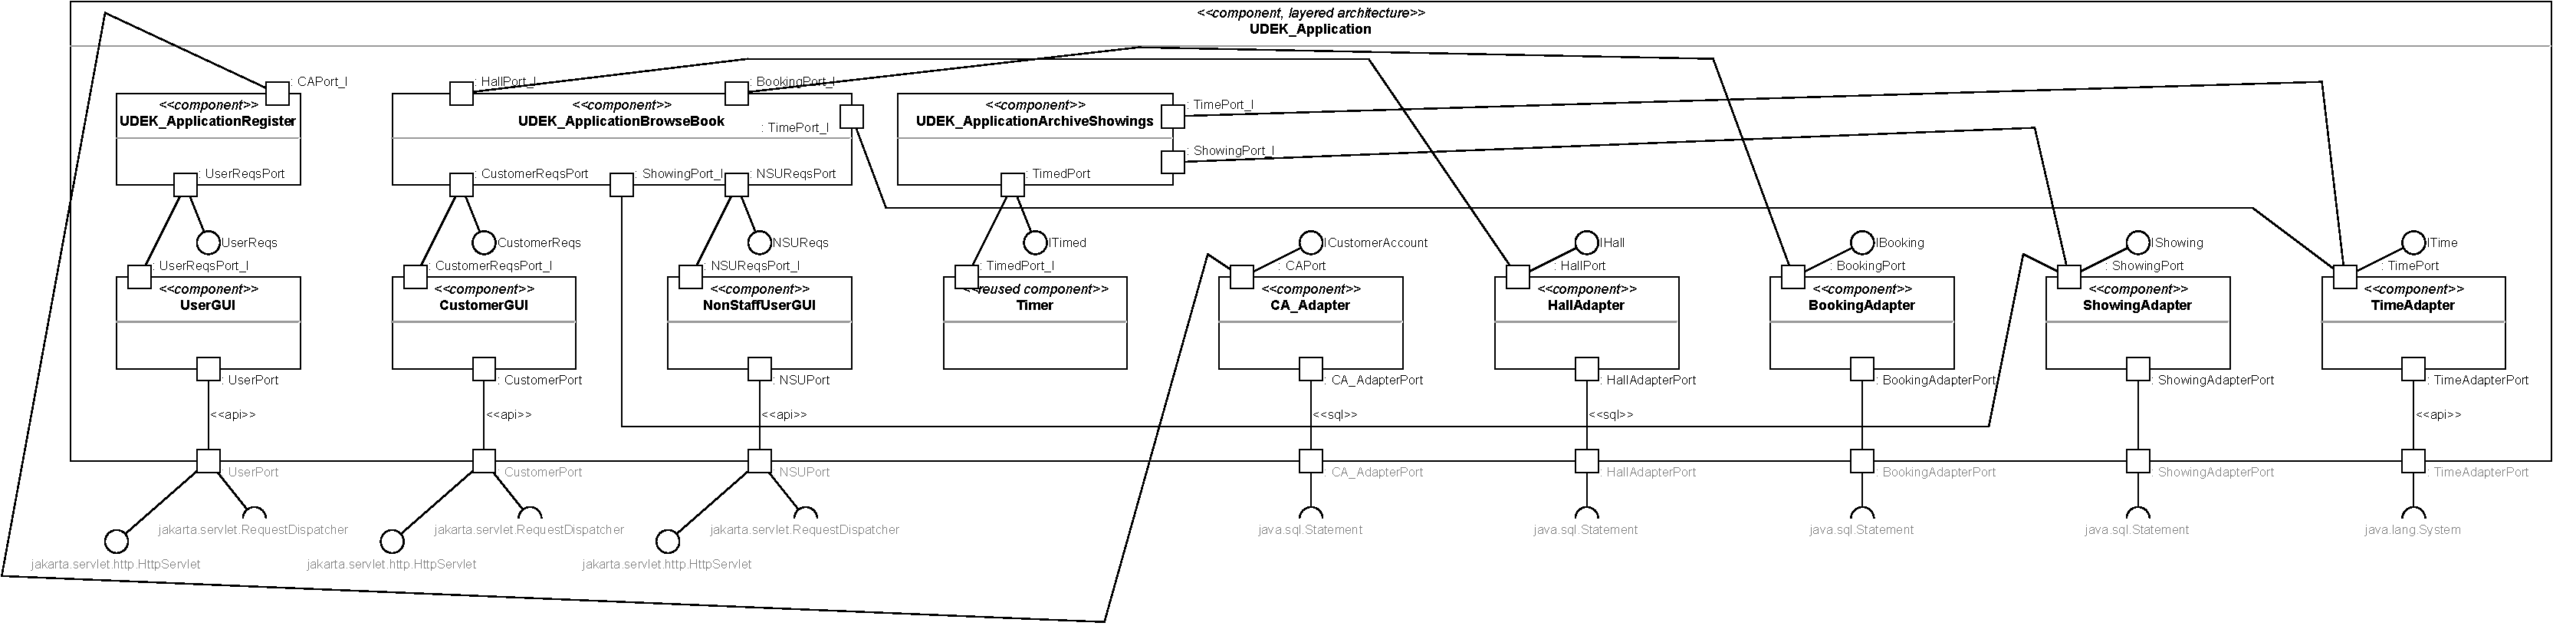
\includegraphics[width = \textwidth]{figures/08/A08_global_architecture.pdf}
    \caption{Global architecture}
    \label{figure:global_architecture}
\end{figure}

\section{D2}

\section{D3}

\section{D4}

State diagrams with tikZ:
%Do not change, only declaration of the element
\tikzstyle{startpoint} = [circle, minimum width=0.5cm, minimum height=0.5cm, text centered, draw=black, fill=black]
\tikzstyle{endpoint} = [circle, minimum width=0.5cm, minimum height=0.5cm, text centered, draw=black, fill=white]
\tikzstyle{endin} = [circle, minimum width=0.05cm, minimum height=0.05cm, text centered, draw=black, fill=black]
\tikzstyle{state} = [rectangle, rounded corners, minimum width=2cm, minimum height=1cm, text centered, draw=black]
\tikzstyle{decision} = [diamond, minimum width=0.5cm, minimum height=0.5cm, text centered, draw=black]
\tikzstyle{arrow} = [->,>=stealth]

\tikzstyle{every node} = [font=\tiny]

%--------------
%--------------We use the same figure environment as for pictures to reference diagrams with tikz.
%--------------Here we provide a small example how to draw a state machine with tikZ.
%--------------The picture is created only with this commands.
%--------------
\begin{figure}[H]
\caption{Zustandsdiagramm Person 1}
\label{d1:zustand1}
\begin{tikzpicture}[node distance=2cm]

%Knoten
\node (Start) [startpoint]{};
\node (State1) [state, right= of Start] {State 1};
\draw [arrow] (Start) -- (State1);

\node (Decision1) [decision, right= of State1]{};
\draw [arrow] (State1) -- (Decision1)  node [pos=0.5,below,fill=white] {Annotation};

\node (State2) [state, below= of Decision1] {State 2};
\draw [arrow] (Decision1) -- (State2)  node [pos=0.2,below,fill=white] {true};



\node (End) [endpoint,right= of State2]{\begin{tikzpicture}\node (End) [endin]{};\end{tikzpicture}};
\draw [arrow] (State2) -- (End);
\draw [arrow] (Decision1) -| (End)  node [pos=0.2,left,fill=white] {false};
\end{tikzpicture}
\end{figure}



\chapter{Implementation \& Testing}

%---------------
%---------------You do not have to copy your source code.
%---------------Just use the given space to add any comments or explanations.
%---------------

\section{I}

\section{T1}

\section{T2}

\section{T3}




%-------------------------
%-------------------------
%--------The glossary makes use of the package longtable to allow automatic page breaks
%-------------------------
%-------------------------
\chapter{Glossary}

\begin{longtable}{|p{.4\linewidth}|p{.2\linewidth}|p{.2\linewidth}|p{.2\linewidth}|}
\caption{Glossary}
\label{table:glossar}\\
\hline
\rowcolor{black!25}\textbf{Name} & \textbf{Type} & \textbf{Description} & \textbf{Source}\\
\hline
\endfirsthead
\caption[]{Glossary}\\
\hline
\rowcolor{black!25}\textbf{Name} & \textbf{Type} & \textbf{Description} & \textbf{Source}\\
\endhead
\hline
\endfoot
\multicolumn{4}{|l|}{\textbf{A}}\\
\hline
\hypertarget{glossary:addBooking}{addBooking} & phenomenon & the \hyperlink{glossary:UDEKino}{machine} adds a new booking to the \hyperlink{glossary:Booking}{bookings database} & CD\\
\hline
addBooking & message & contains a showing ID and seats & SD R5\\
\hline
\hypertarget{glossary:addCustomerAccount}{addCustomerAccount} & phenomenon & the \hyperlink{glossary:UDEKino}{machine} adds a new \hyperlink{glossary:Customer}{customer} to the \hyperlink{glossary:CustomerAccount}{customer accounts database} & CD\\
\hline
addCustomerAccount & message & contains an e-mail address and a password & SD R\ref{enum:R1}\\
\hline
\hypertarget{glossary:addShowing}{addShowing} & phenomenon & the \hyperlink{glossary:UDEKino}{machine} adds a new showing to the \hyperlink{glossary:ShowingsDatabase}{customer accounts database} & CD\\
\hline
APIProvided & class & a class containing various auxiliary functions provided by the runtime environment & Class Model\\
\hline
api & class call name & an instance of the APIProvided class & Class Model\\
\hline
ApacheTomcat & connection domain & An Open Source JSP and Servlet Container from the Apache Foundation. & TCD\\
\hline
addCustomerAccount & phenomenon & creates a CustomerAccount with the provided email and password and adds it to the database & internal interfaces / port types and interface relations RegisterCustomer; app\_if\\
\hline
addBooking & phenomenon & creates a Booking for the customer/showing with the provided email/ID for the provided seat and adds it to the database & internal interfaces / port types and interface relations BookTickets; app\_if\\
\hline
archive & phenomenon & sets the showing with the provided ID to archived & internal interfaces ArchiveShowings; app\_if\\
\hline
%-------------------------
%-------------------------
%--------Each element of the table is expressed in the following way:
%--------Cells are divided by & and each row ends with \\ (linebreak).
%--------The line between two rows is added with \hline.
%-------------------------
%-------------------------
%-------------------------
%-------------------------
\multicolumn{4}{|l|}{\textbf{B}}\\
\hline
\hypertarget{glossary:Booking}{Booking} & lexical domain, designed domain & a database containing the bookings made by \hyperlink{glossary:Customer}{customers} & CD\\
\hline
Booking & object & the database containing all bookings & SD R5\\
\hline
Booking & class & a record representing a booking of a seat for a showing & Class Model\\
\hline
BookingExists & state predicate & given booking exists within the Booking database & SD R5\\
\hline
\hypertarget{glossary:bookingFailed}{bookingFailed} & phenomenon & \hyperlink{glossary:UDEKino}{the machine} notifies \hyperlink{glossary:WebpageBookTickets}{the webpage} that a booking has failed & PD R\ref{enum:R5}\\
\hline
bookingFailed & message & informs the WebpageBookTickets that the booking failed & SD R5\\
\hline
bookingFailed() & method & displays a notification to the customer that the booking failed & Class Model\\
\hline
\hypertarget{glossary:bookingFailedNotification}{bookingFailedNotification} & phenomenon & \hyperlink{glossary:WebpageBookTickets}{the webpage} displays a notification to \hyperlink{glossary:Customer}{the customer} that a booking has failed & PD R\ref{enum:R5}\\
\hline
bookingFailedNotification & message & informs the user that the booking failed & SD R5\\
\hline
bookingIsValid & guard & showing with ID contained in request exists and starts in more than 15 minutes and the seats contained in the request exist in the showing's hall and are not already booked & SD R5\\
\hline
\hypertarget{glossary:bookings}{bookings} & phenomenon & the \hyperlink{glossary:Booking}{bookings database} provides the bookings data to the \hyperlink{glossary:UDEKino}{machine} & CD\\
\hline
bookings & class call name & the database of bookings & Class Model\\
\hline
bookings & message & all bookings in the Booking database & PD R5\\
\hline
\hypertarget{glossary:bookingSuccess}{bookingSuccess} & phenomenon & \hyperlink{glossary:UDEKino}{the machine} notifies \hyperlink{glossary:WebpageBookTickets}{the webpage} that a booking has succeeded & PD R\ref{enum:R5}\\
\hline
bookingSuccess & message & informs the WebpageBookTickets that the booking was successful & SD R5\\
\hline
bookingSuccess() & method & displays a notification to the customer that the booking succeeded & Class Model\\
\hline
\hypertarget{glossary:bookingSuccessNotification}{bookingSuccessNotification} & phenomenon & \hyperlink{glossary:WebpageBookTickets}{the webpage} displays a notification to \hyperlink{glossary:Customer}{the customer} that a booking has succeeded & PD R\ref{enum:R5}\\
\hline
bookingSuccessNotification & message & informs the Customer that the booking was successful & SD R5\\
\hline
\hypertarget{glossary:bookTickets}{bookTickets} & phenomenon & a \hyperlink{glossary:Customer}{customer} books tickets for a showing & CD\\
\hline
BookingAdapter & component & the Booking database adapter & CSD BookTickets\\
\hline
BookingAdapterPort & port & the port connecting the Booking SQL database to its adapter & CSD / port types and interface relations BookTickets\\
\hline
BookingPort & port & the port via which the Booking database may be read and manipulated & CSD / internal interfaces / port types and interface relations BookTickets\\
\hline
BookingPort\_I & port & the port via which the machine reads and manipulates the Booking database & CSD / port types and interface relations BookTickets; app\_if\\
\hline
bookings & phenomenon & the cinema Bookings & port types and interface relations BookTickets\\
\hline
B!{Bookings} & interface & interface from the problem diagram & port types and interface relations BookTickets\\
\hline
CA\_Adapter & component & the CustomerAccount database adapter & CSD RegisterCustomer\\
\hline
CA\_AdapterPort & port & the port connecting the CustomerAccount SQL database to its adapter & CSD / port types and interface relations RegisterCustomer\\
\hline
CAPort & port & the port via which the CustomerAccount database may be read and manipulated & CSD / internal interfaces / port types and interface relations RegisterCustomer\\
\hline
CAPort\_I & port & the port via which the machine reads and manipulates the CustomerAccount database & CSD / internal interfaces / port types and interface relations RegisterCustomer; app\_if\\
\hline
customerAccounts & phenomenon & the customer accounts & internal interfaces / port types and interface relations RegisterCustomer\\
\hline
CA!{customerAccounts} & interface & interface from the problem diagram & port types and interface relations RegisterCustomer\\
\hline
currentDateTime & phenomenon & returns the milliseconds elapsed since the unix epoch & internal interfaces / port types and interface relations BookTickets / ArchiveShowings; app\_if\\
\hline
currentTimeMillis & phenomenon & returns the milliseconds elapsed since the unix epoch & internal interfaces / port types and interface relations BookTickets / ArchiveShowings\\
\hline
CustomerGUI & component & the Customer's gui component & CSD BookTickets\\
\hline
CustomerPort & port & the port to which the servlet container sends requests & CSD / port types and interface relations BookTickets\\
\hline
CustomerReqs & provided interface & an interface to send Customer requests to & CSD / internal interfaces / port types and interface relations BookTickets; app\_if\\
\hline
CustomerReqsPort & port & the machine port to which Customer requests are sent & CSD / internal interfaces / port types and interface relations BookTickets; app\_if\\
\hline
CustomerReqsPort\_I & port & the port to which the CustomerGUI sends Customer requests & CSD / port types and interface relations BookTickets\\
\hline
checkStarted & phenomenon & archives all Showings which have already started & internal interfaces ArchiveShowings; app\_if\\
\hline
\multicolumn{4}{|l|}{\textbf{C}}\\
\hline
\hypertarget{glossary:cBrowse}{cBrowse} & phenomenon & a \hyperlink{glossary:Customer}{customer} browses available showings & CD\\
\hline
checkStarted & found message & a prompt for the UDEK\_ArchiveShowings machine to mark all showings which have already started and are not marked as archived, as archived & SD R7\\
\hline
checkStarted() & methods & archives all showings that start in 15 minutes or less (or already have started) & Class Model\\
\hline
\hypertarget{glossary:cLogin}{cLogin} & phenomenon & a \hyperlink{glossary:User}{user} attempts to log into a \hyperlink{glossary:Customer}{customer} account & CD\\
\hline
\hypertarget{glossary:cLogout}{cLogout} & phenomenon & a \hyperlink{glossary:Customer}{customer} attempts to log out & CD\\
\hline
column & attribute & the column of the booked seat & Class Model\\
\hline
column & parameter & the column of the seat that is to be booked & Class Model\\
\hline
columns & attribute & the number of columns of seats the cinema hall contains & Class Model\\
\hline
\hypertarget{glossary:cRegister}{cRegister} & phenomenon & a \hyperlink{glossary:User}{user} attempts to create customer account on UDEKino & CD\\
\hline
\hypertarget{glossary:cShowWebsite}{cShowWebsite} & phenomenon & the \hyperlink{glossary:UDEKino}{machine} shows a website to the \hyperlink{glossary:Customer}{customer} & CD\\
\hline
currentDateTime() & auxiliary function & returns the current time in unix epoch time & Class Model\\
\hline
\hypertarget{glossary:Customer}{Customer} & biddable domain & a customer of UDEKino; a \hyperlink{glossary:User}{user} who has logged into a customer account & CD. TCD\\
\hline
Customer & actor & a customer who wishes to book tickets & SD R5\\
\hline
customer & attribute & the e-mail address of the customer who made the booking & Class Model\\
\hline
customer & attribute & the e-mail of the session's customer & Class Model\\
\hline
CustomerAccountExists & state predicate & the customer account with the given e-mail address and password exists within the CustomerAccount database & SD R\ref{enum:R1}\\
\hline
\hypertarget{glossary:customerAccounts}{customerAccounts} & phenomenon & the \hyperlink{glossary:CustomerAccount}{customerAccounts database} provides the customerAccounts data to the \hyperlink{glossary:UDEKino}{machine} & CD\\
\hline
customerAccounts & message & all customer accounts in the CustomerAccount database & SD R\ref{enum:R1}\\
\hline
\hypertarget{glossary:CustomerAccount}{CustomerAccount} & lexical domain, designed domain & a database containing \hyperlink{glossary:Customer}{customer} accounts & CD\\
\hline
CustomerAccount & class & a record representing a Customer account & Class Model\\
\hline
customerAccounts & class call name & the database of CustomerAccounts & Class Model\\
\hline
CustomerSession & class & an auxiliary class containing auxiliary functions and data of a logged in Customer's session & Class Model\\
\hline
CustomerWebBrowser & connection domain & Web browser used by a logged in customer, e.g. Mozilla Firefox. & TCD\\
\hline
CustomerAccount & object & the database of customer acccounts & SD R\ref{enum:R1}\\
\hline
\multicolumn{4}{|l|}{\textbf{D}}\\
\hline
\hypertarget{glossary:displayNotification}{displayNotification} & phenomenon & the \hyperlink{glossary:Customer}{customer's} \hyperlink{glossary:Email}{e-mail client} displays a \hyperlink{glossary:notifyCustomer}{notification e-mail} to the \hyperlink{glossary:Customer}{customer} & CD\\
\hline
dateTimeSpanFromMinutes (in minutes : Integer) & auxiliary function & returns the parameter minutes as unix epoch time & Class Model\\
\hline
doGet & technical phenomenon & A procedure called by the \href{https://jakarta.ee/specifications/servlet/}{Jakarta Servlet} container in which the machine can handle an incoming \href{https://datatracker.ietf.org/doc/html/rfc9112}{HTTP} GET request. (See \hyperlink{glossary:forward}{forward}.) & TCD\\
\hline
doPost & technical phenomenon & A procedure called by the \href{https://jakarta.ee/specifications/servlet/}{Jakarta Servlet} container in which the machine can handle an incoming \href{https://datatracker.ietf.org/doc/html/rfc9112}{HTTP} POST request. (See \hyperlink{glossary:forward}{forward}.) & TCD\\
\hline
duration & attribute & the duration of the movie that is to be shown & Class Model\\
\hline
doGet & phenomenon & has the servlet handle the HTTP GET request & port types and interface relations RegisterCustomer / BookTickets / NSUBrowse\\
\hline
doPost & phenomenon & has the servlet handle the HTTP POST request & port types and interface relations RegisterCustomer / BookTickets / NSUBrowse\\
\hline
dateTimeSpanFromMinutes & phenomenon & returns the provided minutes converted to milliseconds & internal interfaces BookTickets; app\_if\\
\hline
\multicolumn{4}{|l|}{\textbf{E}}\\
\hline
\hypertarget{glossary:Email}{Email} & causal domain, connection domain & an e-mail service offering to deliver e-mails & CD\\
\hline
eMailUnused & guard & the e-mail contained in the registration request is not contained in customerAccounts & SD R\ref{enum:R1}\\
\hline
executeQuery & technical phenomenon & A procedure the machine can call to query the contents of a \href{https://www.mysql.com/products/enterprise/techspec.html}{SQL} database. & TCD\\
\hline
executeUpdate & technical phenomenon & A procedure the machine can call to manipulate a \href{https://www.mysql.com/products/enterprise/techspec.html}{SQL} database. & TCD\\
\hline
executeQuery & phenomenon & executes an SQL query & port types and interface relations RegisterCustomer / BookTickets / NSUBrowse\\
\hline
executeUpdate & phenomenon & executes an SQL update & port types and interface relations RegisterCustomer / BookTickets / NSUBrowse\\
\hline
\multicolumn{4}{|l|}{\textbf{F}}\\
\hline
\hypertarget{glossary:forward}{forward} & technical phenomenon & An assortment of procedures and manipulable resources the machine can use to prepare \href{https://datatracker.ietf.org/doc/html/rfc9112}{HTTP} responses which are then sent by the \href{https://jakarta.ee/specifications/servlet/}{Jakarta Servlet} container. & TCD\\
\hline
\hypertarget{glossary:forwardNSUBrowse}{forwardNSUBrowse} & phenomenon & \hyperlink{glossary:WebPageNonStaffUserBrowse}{the website} sends a request for a list of upcoming showings to \hyperlink{glossary:UDEK-NonStaffUserBrowse}{the machine} & PD R\ref{enum:R4} / R\ref{enum:R8}\\
\hline
forwardNSUBrowse() & method & the machine handles the browse request & Class Model\\
\hline
forwardNSUBrowse & message & a request for the machine to send a list of available, i.e., non-archived, showings & SD R4/8\\
\hline
\hypertarget{glossary:forwardSubmitBooking}{forwardSubmitBooking} & phenomenon & \hyperlink{glossary:WebpageBookTickets}{the webpage} forwards a request to book tickets to \hyperlink{glossary:UDEKino}{the machine} & PD R\ref{enum:R5}\\
\hline
forwardSubmitRegistration() & method & the machine handles the registration request: it creates a new account if possible and sends a status notification to the webpage & Class Model\\
\hline
forwardSubmitBooking & message & contains the showing ID and the desired seats & SD R5\\
\hline
forwardSubmitBooking & method & tries to book the given seat for the given showing and informs the webpage of the success or failure afterwards & Class Model\\
\hline
\hypertarget{glossary:forwardSubmitRegistration}{forwardSubmitRegistration} & phenomenon & \hyperlink{glossary:WebpageRegisterCustomer}{the webpage} forwards a request to register a \hyperlink{glossary:Customer}{customer account} to \hyperlink{glossary:UDEKino}{the machine} & PD R\ref{enum:R1}\\
\hline
forwardSubmitRegistration & message & a request from the WebpageRegisterCustomer to register a new customer account, containing an e-mail address and a password & SD R\ref{enum:R1}\\
\hline
forwardSubmitRegistration & phenomenon & forwards a registration request to the responsible component, returns registrationSuccess or registration Failed depending on whether the registration succeeded or failed & internal interfaces / port types and interface relations RegisterCustomer; app\_if\\
\hline
forwardSubmitBooking & phenomenon & forwards a booking request to the responsible component, returns bookingSuccess or booking Failed depending on whether the booking succeeded or failed & internal interfaces / port types and interface relations BookTickets; app\_if\\
\hline
forwardNSUBrowse & phenomenon & forwards a browse request to the responsible component, returns all currently available showings & internal interfaces / port types and interface relations NSUBrowse; app\_if\\
\hline
\multicolumn{4}{|l|}{\textbf{G}}\\
\hline
get\_bookings & message & contains all messages in the Booking database & SD R5\\
\hline
get\_customerAccounts & message & returns all customer accounts in the CustomerAccount database & SD R\ref{enum:R1}\\
\hline
get\_halls & message & returns all halls in the Hall database & SD R5\\
\hline
get\_showings & message & returns all showings in the Showing database & SD R5, 4/8, 7\\
\hline
gui & technical phenomenon & The web browser renders a webpage. & TCD\\
\hline
getCustomerAccount & phenomenon & returns the CustomerAccount with the given email, if it exists & internal interfaces RegisterCustomer; app\_if\\
\hline
getHall & phenomenon & returns the Hall with the given hallNumber, if it exists & internal interfaces BookTickets; app\_if\\
\hline
getShowing & phenomenon & returns the Showing with the given ID, if it exists & internal interfaces BookTickets; app\_if\\
\hline
getShowings & phenomenon & returns all Showings & internal interfaces Browse / ArchiveShowings; app\_if\\
\hline
getBooking & phenomenon & returns the Booking for the given showing and seat, if it exists & internal interfaces BookTickets; app\_if\\
\hline
\multicolumn{4}{|l|}{\textbf{H}}\\
\hline
Hall & object & the database containing the cinema halls & SD R5\\
\hline
Hall & class & a record representing a cinema hall & Class Model\\
\hline
hallNumber & attribute & the number of the hall the showing will take place in & Class Model\\
\hline
\hypertarget{glossary:halls}{halls} & phenomenon & the \hyperlink{glossary:Hall}{halls database} provides the halls data to the \hyperlink{glossary:UDEKino}{machine} & CD\\
\hline
halls & message & all halls in the Hall database & SD R5\\
\hline
halls & class call name & the database of cinema halls & Class Model\\
\hline
\hypertarget{glossary:Hall}{Hall} & lexical domain & a database containing the cinema halls, provided by the cinema operator & CD\\
\hline
http & technical phenomenon & The \href{https://datatracker.ietf.org/doc/html/rfc9112}{Hypertext Transfer Protocol}. A client-server protocol for requesting and providing data, like webpages, over the internet. & TCD\\
\hline
HallAdapter & component & the Hall database adapter & CSD BookTickets\\
\hline
HallAdapterPort & port & the port connecting the Hall SQL database to its adapter & CSD / port types and interface relations BookTickets\\
\hline
HallPort & port & the port via which the Hall database may be read & CSD / internal interfaces / port types and interface relations BookTickets\\
\hline
HallPort\_I & port & the port via which the machine reads the Hall database & CSD / port types and interface relations BookTickets; app\_if\\
\hline
halls & phenomenon & the cinema halls & port types and interface relations BookTickets\\
\hline
H!{halls} & interface & interface from the problem diagram & port types and interface relations BookTickets\\
\hline
\multicolumn{4}{|l|}{\textbf{I}}\\
\hline
id & attribute & the unique id of the showing & Class Model\\
\hline
id & attribute & the unique ID of the booking & Class Model\\
\hline
imap & technical phenomenon & \href{https://tools.ietf.org/html/rfc3501}{Internet Message Access Protocol} & TCD\\
\hline
isArchived & attribute & indicates whether the showing is archived & Class Model\\
\hline
ICustomerAccount & provided interface & an interface via which the CustomerAccount database may be read and manipulated & CSD / internal interfaces / port types and interface relations RegisterCustomer; app\_if\\
\hline
IHall & provided interface & an interface via which the Hall database may be read & CSD / internal interfaces / port types and interface relations BookTickets; app\_if\\
\hline
IBooking & provided interface & an interface via which the Booking database may be read and manipulated & CSD / internal interfaces / port types and interface relations BookTickets; app\_if\\
\hline
IShowing & provided interface & an interface via which the Showing database may be read and manipulated & CSD / internal interfaces / port types and interface relations BookTickets / Browse / ArchiveShowings; app\_if\\
\hline
ITime & provided interface & an interface for providing time related utilities & CSD / internal interfaces / port types and interface relations BookTickets / ArchiveShowings; app\_if\\
\hline
ITimed & provided interface & an interface for triggering timed internal actions & CSD / internal interfaces / port types and interface relations ArchiveShowings; app\_if\\
\hline
\multicolumn{4}{|l|}{\textbf{J}}\\
\hline
jakarta.servlet.http.Servlet & provided interface & provides handling of HTTP requests & CSD / port types and interface relations RegisterCustomer / BookTickets / NSUBrowse\\
\hline
jakarta.servlet.RequestDispatcher & required interface & a interface to which HTTP requests may be forwarded & / port types and interface relations CSD RegisterCustomer / BookTickets / NSUBrowse\\
\hline
java.sql.Statement & required interface & an interface for executing SQL statements & CSD / port types and interface relations RegisterCustomer / BookTickets / NSUBrowse\\
\hline
java.lang.System & required interface & an interface for executing SQL statements & CSD / port types and interface relations BookTickets / ArchiveShowings\\
\hline
\multicolumn{4}{|l|}{\textbf{K}}\\
\hline
&  &  & \\
\hline
\multicolumn{4}{|l|}{\textbf{L}}\\
\hline
LC\_{User} & life-cycle & Life-cycle for one user & LC\\
\hline
LC\_{Customer} & life-cycle & Life-cycle for one logged in customer & LC\\
\hline
LC\_{NonStaffUser} & life-cycle & Life-cycle for one user who is not logged in as staff & LC\\
\hline
LC\_{UDEKino} & life-cycle & Combined life-cycle (all users, customers and internal operations) & LC\\
\hline
\multicolumn{4}{|l|}{\textbf{M}}\\
\hline
MailClient & connection domain & the Customer's E-Mail client & TCD\\
\hline
MailServerCustomer & connection domain & the customer's E-Mail server & TCD\\
\hline
MailServerUDEK & connection domain & the system's E-Mail server & TCD\\
\hline
minutes & parameter & the minutes to be converted to unix epoch time & Class Model\\
\hline
\hypertarget{glossary:modifyShowing}{modifyShowing} & phenomenon & \hyperlink{glossary:UDEKino}{the machine} modifies a showing in the \hyperlink{glossary:Showing}{showings database} & CD\\
\hline
modifyShowing & phenomenon & modifies a showing & port tyypes and interface relations ArchiveShowings\\
\hline
\multicolumn{4}{|l|}{\textbf{N}}\\
\hline
\hypertarget{glossary:NonStaffUser}{NonStaffUser} & biddable domain & either of \hyperlink{glossary:Customer}{Customer} or \hyperlink{glossary:User}{User} & PD R\ref{enum:R4} / R\ref{enum:R8}\\
\hline
NonStaffUser & actor & a user who is not logged in as staff and wishes to browse available showings & SD R4/8\\
\hline
\hypertarget{glossary:notifyCustomer}{notifyCustomer} & phenomenon & the \hyperlink{glossary:UDEKino}{machine} notifies the \hyperlink{glossary:Customer}{customer} via \hyperlink{glossary:Email}{e-mail} & CD\\
\hline
\hypertarget{glossary:nsuBrowse}{nsuBrowse} & phenomenon & either of \hyperlink{glossary:cBrowse}{cBrowse} or \hyperlink{glossary:uBrowse}{uBrowse} & PD R\ref{enum:R4} / R\ref{enum:R8}\\
\hline
nsuBrowse & message & a request for the WebpageNonStaffUserBrowse to display available showings & SD R4/8\\
\hline
nsuBrowse() & method & the user requests a list of available showings on the webpage & Class Model\\
\hline
\hypertarget{glossary:nsuShowings}{nsuShowings} & phenomenon & \hyperlink{glossary:UDEK-NonStaffUserBrowse}{the machine} sends a list of upcoming showings to be displayed by \hyperlink{glossary:WebPageNonStaffUserBrowse}{the website} & PD R\ref{enum:R4} / R\ref{enum:R8}\\
\hline
nsuShowings & message & contains available, i.e., non-archived, showings & SD R4/8\\
\hline
nsuShowings() & method & the machine sends a set of available showings to the webpage & Class Model\\
\hline
\hypertarget{glossary:nsuShowShowings}{nsuShowShowings} & phenomenon & \hyperlink{glossary:WebPageNonStaffUserBrowse}{the website} displays a list of upcoming showings to the \hyperlink{glossary:NonStaffUser}{user} & PD R\ref{enum:R4} / R\ref{enum:R8}\\
\hline
nsuShowShowings & message & a rendition of available, i.e., non-archived, showings & SD R4/8\\
\hline
NonStaffUserGUI & component & the NonStaffUser's gui component & CSD RegisterCustomer\\
\hline
NSUPort & port & the port to which the servlet container sends requests & CSD / port types and interface relations RegisterCustomer\\
\hline
NSUReqs & provided interface & an interface to send NonStaffUser requests to & CSD / internal interfaces / port types and interface relations RegisterCustomer; app\_if\\
\hline
NSUReqsPort & port & the machine port to which NonStaffUser requests are sent & CSD / internal interfaces / port types and interface relations RegisterCustomer; app\_if\\
\hline
NSUReqsPort\_I & port & the port to which the NonStaffUserGUI sends NonStaffUser requests & CSD / port types and interface relations RegisterCustomer\\
\hline
\hline
\multicolumn{4}{|l|}{\textbf{O}}\\
\hline
&  &  & \\
\hline
\multicolumn{4}{|l|}{\textbf{P}}\\
\hline
pop3 & technical phenomenon & \hyperlink{tools.ietf.org/html/rfc1939}{Post Office Protocol - Version 3} & \\
\hline
\multicolumn{4}{|l|}{\textbf{Q}}\\
\hline
&  &  & \\
\hline
\multicolumn{4}{|l|}{\textbf{R}}\\
\hline
\hypertarget{glossary:registrationFailed}{registrationFailed} & phenomenon & \hyperlink{glossary:UDEKino}{the machine} notifies \hyperlink{glossary:WebpageRegisterCustomer}{the webpage} that the registration has failed & PD R\ref{enum:R1}\\
\hline
registrationFailed & message & informs the WebpageRegisterCustomer that account creation has failed & SD R\ref{enum:R1}\\
\hline
registrationFailed() & method & the webpage is notified that the registration was successful & Class Model\\
\hline
\hypertarget{glossary:registrationFailedNotification}{registrationFailedNotification} & phenomenon & \hyperlink{glossary:WebpageRegisterCustomer}{the webpage} displays a to \hyperlink{glossary:User}{the user} that the registration has failed & PD R\ref{enum:R1}\\
\hline
registrationFailedNotification & message & informs the user that account creation has succeeded & SD R\ref{enum:R1}\\
\hline
\hypertarget{glossary:registrationSuccess}{registrationSuccess} & phenomenon & \hyperlink{glossary:UDEKino}{the machine} notifies \hyperlink{glossary:WebpageRegisterCustomer}{the webpage} that the registration has succeeded & PD R\ref{enum:R1}\\
\hline
registrationSuccess & message & informs the WebpageRegisterCustomer that account registration has succeeded & SD R\ref{enum:R1}\\
\hline
registrationSuccess() & method & the webpage is notified that the registration was unsuccessful & Class Model\\
\hline
\hypertarget{glossary:registrationSuccessNotification}{registrationSuccessNotification} & phenomenon & \hyperlink{glossary:WebpageRegisterCustomer}{the webpage} displays a notification to \hyperlink{glossary:User}{the user} that the registration has succeeded & PD R\ref{enum:R1}\\
\hline
registrationSuccessNotification & message & informs the User that account creation has succeeded & SD R\ref{enum:R1}\\
\hline
\hypertarget{glossary:removeBooking}{removeBooking} & phenomenon &  \hyperlink{glossary:UDEKino}{the machine} removes a booking from the \hyperlink{glossary:Booking}{bookings database} & CD\\
\hline
\hypertarget{glossary:removeBooking}{removeCustomer} & phenomenon &  \hyperlink{glossary:UDEKino}{the machine} removes a \hyperlink{glossary:Customer}{customer} from the \hyperlink{glossary:CustomerAccount}{customers database} & CD\\
\hline
\hypertarget{glossary:removeShowing}{removeShowing} & phenomenon &  \hyperlink{glossary:UDEKino}{the machine} removes a showing from the \hyperlink{glossary:Showing}{showings database} & CD\\
\hline
row & attribute & the row of the booked seat & Class Model\\
\hline
row & parameter & the row of the seat that is to be booked & Class Model\\
\hline
rows & attribute & the number of rows of seats the cinema hall contains & Class Model\\
\hline
result & parameter & the set of available showings & Class Model\\
\hline
registrationSuccess & phenomenon & informs the webpage that the registration succeded & port types and interface relations RegisterCustomer\\
\hline
registrationFailed & phenomenon & informs the webpage that the registration failed & port types and interface relations RegisterCustomer\\
\hline
\multicolumn{4}{|l|}{\textbf{S}}\\
\hline
\hypertarget{glossary:sBrowse}{sBrowse} & phenomenon & a \hyperlink{glossary:StaffMember}{staff member} browses available showings & CD\\
\hline
\hypertarget{glossary:sCancelShowing}{sCancelShowing} & phenomenon & a \hyperlink{glossary:StaffMember}{staff member} attempts to cancel a showing & CD\\
\hline
send & technical phenomenon & the machine sends an e-mail & TCD\\
\hline
session & class call name & the request's session & Class Model\\
\hline
setArchived & message & contains the ID of the showing which is to be marked as archived & SD R7\\
\hline
\hypertarget{glossary:Showing}{Showing} & lexical domain, designed domain & a database containing the cinema showings & CD\\
\hline
Showing & object & the database containing the showings & SD R5, 4/8, 7\\
\hline
Showing & class & a record representing a showing & Class Model\\
\hline
ShowingHasStarted & guard / state predicate & whether the showing in question has already started, i.e., its starting date and time lies in the past & SD R7\\
\hline
showingID & attribute & the ID of the showing of the booking & Class Model\\
\hline
showingID & parameter & the ID of the showing that is to be booked & Class Model\\
\hline
ShowingIsArchived & guard / state predicate & whether the showing in question is marked as archived" & SD R7\\
\hline
\hypertarget{glossary:showings}{showings} & phenomenon & the \hyperlink{glossary:Showing}{showings database} provides the showings data to the \hyperlink{glossary:UDEKino}{machine} & CD\\
\hline
showings & message & contains all showings in the Showing database & SD R5, 4/8, 7\\
\hline
showings & class call name & the database of Showings & Class Model\\
\hypertarget{glossary:sLogin}{sLogin} & phenomenon & a \hyperlink{glossary:User}{user} attempts to log in as a \hyperlink{glossary:StaffMember}{staff member} & CD\\
\hline
\hypertarget{glossary:sLogout}{sLogout} & phenomenon & a \hyperlink{glossary:StaffMember}{staff member} attempts to log out & CD\\
\hline
SMTP & technical phenomenon & \href{http://tools.ietf.org/html/rfc2821}{Simple Mail Transfer Protocol} & TCD\\
\hline
\hypertarget{glossary:sShowWebsite}{sShowWebsite} & phenomenon & the \hyperlink{glossary:UDEKino}{machine} shows a website to the \hyperlink{glossary:StaffMember}{staff member} & CD\\
\hline
\hypertarget{glossary:StaffMember}{StaffMember} & biddable domain & a member of cinema staff; a \hyperlink{glossary:User}{user} who has logged in as staff & CD\\
\hline
startDateTime & attribute & the date and time the showing will start at in unix epoch time & Class Model\\
\hline
\hypertarget{glossary:submitBooking}{submitBooking} & phenomenon & the \hyperlink{glossary:Customer}{customer} selects the tickets they wish to book and hits the submit button &  PD R\ref{enum:R5}\\
\hline
submitBooking & message & contains the showing ID and desired seats & SD R5\\
\hline
submitBooking(in showingID : Integer, in row : Integer, in column : Integer) & method & forwards the booking request to the machine & Class Model\\
\hline
\hypertarget{glossary:submitRegistration}{submitRegistration} & phenomenon & the \hyperlink{glossary:User}{user} submits a request to register a new \hyperlink{glossary:Customer}{customer} account, containing an e-mail address and a password & PD R\ref{enum:R1}\\
\hline
submitRegistration & message & a request from the user to register a new customer account, containing an e-mail address and a password & SD R\ref{enum:R1}\\
\hline
submitRegistration(in email : String, in password : String) & method & the method with which the user submits the registration form & Class Model\\
\hline
\hypertarget{glossary:submitShowing}{submitShowing} & phenomenon & a \hyperlink{glossary:StaffMember}{staff member} submits a new showing to the machine for entry into the database & CD\\
\hline
ShowingAdapter & component & the Showing database adapter & CSD BookTickets / NUSBrowse / ArchiveShowings\\
\hline
ShowingAdapterPort & port & the port connecting the Showing SQL database to its adapter & CSD / port types and interface relations BookTickets / NUSBrowse / ArchiveShowings\\
\hline
ShowingPort & port & the port via which the Showing database may be read and manipulated & CSD / internal interfaces / port types and interface relations BookTickets / NUSBrowse / ArchiveShowings\\
\hline
ShowingPort\_I & port & the port via which the machine reads and manipulates the Showing database & CSD / port types and interface relations BookTickets / NUSBrowse / ArchiveShowings; app\_if\\
\hline
showings & phenomenon & the cinema Showings & port types and interface relations BookTickets / NUSBrowse / ArchiveShowings\\
\hline
S!{showings} & interface & interface from the problem diagram & port types and interface relations BookTickets / NUSBrowse / ArchiveShowings\\
\hline
\multicolumn{4}{|l|}{\textbf{T}}\\
\hline
TimeAdapter & component & an adapter providing time related utilities & CSD / internal interfaces / port types and interface relations BookTickets / ArchiveShowings\\
\hline
TimeAdapterPort & port & the port providing system time to the time adapter & CSD / internal interfaces / port types and interface relations BookTickets / ArchiveShowings\\
\hline
TimeAdapterPort\_I & port & the port consuming system time & CSD / internal interfaces / port types and interface relations BookTickets / ArchiveShowings\\
\hline
TimePort & port & the port providing time related utilities & CSD / internal interfaces / port types and interface relations BookTickets / ArchiveShowings\\
\hline
TimePort\_I & port & the port consuming time related utilities & CSD / internal interfaces / port types and interface relations BookTickets / ArchiveShowings; app\_if\\
\hline
Timer & component & a timer triggering certain actions in certain intervals & CSD ArchiveShowings\\
\hline
TimedPort & port & the machine port for triggering timed internal actions & CSD / internal interfaces ArchiveShowings; app\_if\\
\hline
TimedPort\_I & port & the port which triggers timed internal actions & CSD / internal interfaces ArchiveShowings\\
\hline
\multicolumn{4}{|l|}{\textbf{U}}\\
\hline
\hypertarget{glossary:uBrowse}{uBrowse} & phenomenon & a \hyperlink{glossary:User}{user} browses available showings & CD\\
\hline
\hypertarget{glossary:UDEKino}{UDEKino} & machine & the machine to be developed & CD, TCD\\
\hline
\hypertarget{glossary:UDEK-ArchiveShowings}{UDEK\_ArchiveShowings} & machine & the sub-\hyperlink{glossary:UDEKino}{machine} responsible for automatically archiving showings once they have begun & PD R\ref{enum:R7} \\
\hline
UDEK\_ArchiveShowings & object & the sub-machine responsible for archiving showings which have already started & SD R7\\
\hline
UDEK\_ArchiveShowings & class & the machine class & Class Model\\
\hline
\hypertarget{glossary:UDEK-BookTickets}{UDEK\_BookTickets} & machine & the sub-\hyperlink{glossary:UDEKino}{machine} responsible for \hyperlink{glossary:Customer}{customer} booking tickets & PD R\ref{enum:R5}\\
\hline
UDEK\_BookTickets & object & the machine responsible for the booking of tickets & SD R5\\
\hline
UDEK\_BookTickets & class & the machine class & Class Model\\
\hline
udek\_bookTickets & class call name & the machine class intance & Class Model\\
\hline
\hypertarget{glossary:UDEK-NonStaffUserBrowse}{UDEK\_NonStaffUserBrowse} & machine & the sub-\hyperlink{glossary:UDEKino}{machine} responsible for \hyperlink{glossary:NonStaffUser}{registered and non-registered} customers browsing upcoming showings & PD R\ref{enum:R4} / R\ref{enum:R8}\\
\hline
UDEK\_NonStaffUserBrowse & class & the machine class & Class Model\\
\hline
udek\_NonStaffUserBrowse & class call name & the instance of the machine class the webpage belongs to & Class Model\\
\hline
\hypertarget{glossary:UDEK-RegisterCustomer}{UDEK\_RegisterCustomer} & machine & the sub-\hyperlink{glossary:UDEKino}{machine} responsible for \hyperlink{glossary:Customer}{customer} account registration & PD R\ref{enum:R1}\\
\hline
UDEK\_RegisterCustomer & object & the machine responsible for customer account registration & SD R\ref{enum:R1}\\
\hline
UDEK\_RegisterCustomer & class & the machine class & Class Model\\
\hline
udek\_registerCustomer & class call name & the instance of the machine class the webpage belongs to & Class Model\\
\hline
\hypertarget{glossary:User}{User} & biddable domain & a user of the \hyperlink{glossary:UDEKino}{application} who is not logged in & CD, TCD\\
\hline
UserWebBrowser & connection domain & Web browser used by a user who is not logged in, e.g. Mozilla Firefox. & TCD\\
\hline
User & actor & a user of who wishes to register a new customer account & SD R\ref{R1}\\
\hline
\hypertarget{glossary:uShowWebsite}{uShowWebsite} & phenomenon & the \hyperlink{glossary:UDEKino}{machine} shows a website to the \hyperlink{glossary:User}{user} & CD\\
\hline
UDEK\_Application & component & the application component & CSD RegisterCustomer / BookTickets / NSUBrowse\\
\hline
UDEK\_RegisterCustomer & machine & the machine component & CSD RegisterCustomer\\
\hline
UDEK\_BooKTickets & machine & the machine component & CSD BookTickets\\
\hline
UDEK\_NonStaffUserBrowse & machine & the machine component & CSD NonStaffUserBrowse\\
\hline
UserGUI & component & the User's gui component & CSD RegisterCustomer\\
\hline
UserPort & port & the port to which the servlet container sends requests & CSD / port types and interface relations RegisterCustomer\\
\hline
UserReqs & provided interface & an interface to send user requests to & CSD / internal interfaces / port types and interface relations RegisterCustomer; app\_if\\
\hline
UserReqsPort & port & the machine port to which user requests are sent & CSD / internal interfaces / port types and interface relations RegisterCustomer; app\_if\\
\hline
UserReqsPort\_I & port & the port to which the UserGUI sends user requests & CSD / port types and interface relations RegisterCustomer\\
\hline
UDEK\_RC!\{registrationSuccess, registrationFailed\} & interface & interface from the problem diagram & port types and interface relations RegisterCustomer\\
\hline
UDEK\_RC!\{addCustomerAccount\} & interface & interface from the problem diagram & port types and interface relations RegisterCustomer\\
\hline
UDEK\_BT!\{bookingSuccess, bookingFailed\} & interface & interface from the problem diagram & port types and interface relations BookTickets\\
\hline
UDEK\_BT!\{addBooking\} & interface & interface from the problem diagram & port types and interface relations BookTickets\\
\hline
UDEK\_NSUB!\{nsuShowings\} & interface & interface from the problem diagram & port types and interface relations NSUBrowse\\
\hline
UDEK\_AS!\{modifyShowing\} & interface & interface from the problem diagram & port types and interface relations ArchiveShowings\\
\hline
\multicolumn{4}{|l|}{\textbf{V}}\\
\hline
&  &  & \\
\hline
\multicolumn{4}{|l|}{\textbf{W}}\\
\hline
\hypertarget{glossary:WebpageBookTickets}{WebpageBookTickets} & connection domain, designed domain & a webpage via which a \hyperlink{glossary:Customer}{customer} can book tickets & PD R\ref{enum:R5}\\
\hline
WebpageBookTickets & object & the webpage for booking tickets & SD R5\\
\hline
WebpageBookTickets & class & the class of the webpage for the booking of tickets & Class Model\\
\hline
webpageBookTickets & class call name & the webpage via which the request was sent & Class Model\\
\hline
\hypertarget{glossary:WebpageNonStaffUserBrowse}{WebpageNonStaffUserBrowse} & connection domain, designed domain & a webpage via which a \hyperlink{glossary:NonStaffUser}{user} can browse upcoming showings & PD R\ref{enum:R4} / R\ref{enum:R8}\\
\hline
WebpageNonStaffUserBrowse & object & the webpage for NonStaffUsers to browse available showings & SD R4/8\\
\hline
WebpageNonStaffUserBrowse & class & the class representing the webpage for browsing showings & Class Model\\
\hline
webpageNonStaffUserBrowse & class call name & the webpage instance whose request is currently being handled & Class Model\\
\hline
\hypertarget{glossary:WebpageRegisterCustomer}{WebpageRegisterCustomer} & connection domain, designed domain & a webpage via which a \hyperlink{glossary:User}{user} can register a new \hyperlink{glossary:Customer}{customer account} & PD R\ref{enum:R1}\\
\hline
WebpageRegisterCustomer & object & the webpage for registering a new customer account & SD R\ref{enum:R1}\\
\hline
WebpageRegisterCustomer & class & the class of the webpage for customer registration & Class Model\\
\hline
webpageRegisterCustomer & class call name & the instance of the registration webpage class whose request is currently being handled & Class Model\\
\hline
WPRC!\{forwardSubmitRegistration\} & interface & interface from the problem diagram & port types and interface relations RegisterCustomer\\
\hline
WPBT!\{forwardSubmitBooking\} & interface & interface from the problem diagram & port types and interface relations BookTickets\\
\hline
WPNSUB!\{forwardNSUBrowse\} & interface & interface from the problem diagram & port types and interface relations NSUBrowse\\
\hline
\multicolumn{4}{|l|}{\textbf{X}}\\
\hline
&  &  & \\
\hline
\multicolumn{4}{|l|}{\textbf{Y}}\\
\hline
&  &  & \\
\hline
\multicolumn{4}{|l|}{\textbf{Z}}\\
\hline
&  &  & \\
\hline
\end{longtable}

\end{document}